\chapter{Feature Engineering}
\label{ch:feature_engineering}
The ultimate goal of `Feature Engineering' is to clean and transform the data
using heuristics and event tagging. Events are tagged to identify tracks which
are likely to originate from signal sources, as separate from events which come
from the background. Subsequently, the signal to background ratio and
longitudinal spin asymmetry are measured.

Even with the Forward Upgrade (Section~\ref{sec:forward_upgrade}), the data set
is still composed mostly of background events. The primary constituents of the
data set are muons from the following sources:

\begin{itemize}
  \item \textbf{Hadronic Background}
    \begin{itemize}
      \item This hadronic background source is composed of hadrons which are
        produced at the primary event vertex, and then travel into the Muon
        Arms. The hadrons then decay into muons in the volume of the Muon Arms.
        The hit pattern from such decays is mis-reconstructed as high-$p_T$
        muons originating at the primary event vertex. Though the probability of
        this scenario is small, the large number of hadrons results in a
        substantial background. 
    \end{itemize}
  \item \textbf{Muon Background}
    \begin{itemize}
        \item The muon background is composed of processes which produce real
          muons which fall into a similar kinematic regime of the W-genic muons.
          This contribution is separated from the signal data set with a
          combination of likelihood event tagging (Section~\ref{sec:likelihood})
          and an unbinned maximum likelihood fit (Section~\ref{sec:sbr}).
    \end{itemize}
  \item \textbf{W Signal}
    \begin{itemize}
        \item These are the original muons from the $W$ Boson decay, and carry
          information about the proton's spin.
    \end{itemize}
\end{itemize}

Likelihood event selection is applied in the first stage of event selection,
where two classifications are considered for muon tracks. The first
classification is `background', which is composed of real muon background, and
mis-reconstructed muon tracks originating from hadronic decay. The second
classification is `signal', which is composed of muons which have a high
likelihood of having decayed from a $W$-Boson, alternatively referred to as
`W-genic' tracks. This process is described in Section~\ref{sec:likelihood}.

The second stage of event selection differentiates the data set into three
classifications--hadronic background, muon background and $W$-Boson decays.
The recorded data set is used as a proxy for the hadronic background, while the
$W$ Boson and Muon Background contributions are modeled with a combination of
simulation of tracks originating from the $W$ Boson and Muon Background
processes, as well as extrapolation from the data set. This is accomplished with
a Maximum Likelihood Fit, described in Section~\ref{sec:sbr}.

In subsequent sections, I will provide a greater context for motivating the
selection of analysis variables. As this data set is dominated by background
sources, the analysis relies heavily on simulations to estimate how signal $\mu$
events might look like in the PHENIX detectors.

At the time of writing, simulation of hadronic background has not yet been
incorporated into the analysis, as there are many effects to consider. For
example, how particles interact with the material of PHENIX to produce secondary
and tertiary vertices. Also, as the percentage of hadronic background events
which mimic W-genic muons is very small, trillions of events need to be
generated. However, it is possible to accurately simulate the signal process,
and the muon background processes, since both know these processes are
understood with high precision.

To form the basis of separating signal and background, the data itself is used
as a proxy for what the `hadronic background' may look like, and the simulations
are used to represent the portions of data which cannot come from this hadronic
background. Even so, it is certain that the $W$ signal must be in the data
sample.

\clearpage
\section{The Basic Cut}
\label{sec:basic_cut}

The basic cut aims to remove all events which are kinematically forbidden from
resulting from a $W$-boson decay. Because the $W$ boson must produce narrowly
curved muons due to high momentum, one may remove tracks outside of a momentum
threshold. The threshold is defined both in terms of the actual reconstructed
momentum, as well as with respect to variables which are correlated to the
amount of track bending.

{\noindent}The ``Basic Cut'' is defined:
\begin{table}[ht]
  \centering
  \begin{tabular}{l c c}
    \toprule
    \textbf{Variable} & \textbf{Lower Bound} & \textbf{Upper Bound} \\
    \midrule
    DG0 & 0 $cm$ & 20 $cm$ \\
    DDG0 & 0.0 $^\circ$ & 9.0 $^\circ$ \\
    DCA$_r$ & 0 $cm$ & 30.0 $cm$ \\
    $\chi^2$ & 0 & 20 \\
    $p$ & 5 $GeV/c$ & 250 $GeV/c$ \\
    $p_T$ & 16 $GeV/c$ & 60 $GeV/c$ \\ 
    $RPC_1DCA$ & 0 $cm$ & 20 $cm$ \\
    $RPC_3DCA$ & 0 $cm$ & 40 $cm$ \\
    $fvtx_{d\theta}$ & 0 $rad$ & 1.5 $rad$ \\
    $fvtx_{d\phi}$ & 0 $rad$ & 1.5 $rad$ \\
    MuID lastGap & Gap 4 & * \\ 
    Number of $\mu$ Tracks Per Event & N/A & 1 \\
    \bottomrule
  \end{tabular}
  \caption{ 
    The Basic Cuts used in the Run 13 analysis. lastGap refers to the last gap
    in the MUID which saw a $\mu$ candidate event. The fourth gap is the
    furthest penetration possible, therefore suggesting a high enough energy
    muon.  Other parameters are described in Tables \ref{tab:evt_variables},
    \ref{tab:mutr_variables}, \ref{tab:fvtx_variables}, and
    \ref{tab:rpc_variables}
  }
  \label{tab:basic_cut}
\end{table}

With this cut, a we reduce the background in our data by a factor of about
15,700--without worry of removing any events in that fall within the kinematic
range of $W$ Boson production. The basic cut reduces our data set from 15.7
billion events to about one million events.

\clearpage
\section{Simulations}

PHENIX has a rather well developed simulation framework, which uses the in-house
built ``PHENIX Integrated Simulation Application'' (PISA)~\cite{Maguire1997}
custom simulation framework. The simulation framework models the entire
12m$\times$18m$\times$18m volume of the PHENIX apparatus in detail, as well as
all the various material properties of the apparatus. The software package uses
GEANT as a basis, with PHENIX geometry build on top. PISA additionally
encapsulates event-generators, a standalone geometry verification package, and
the PHENIX offline analysis shell, in order to generate data that is completely
compatible with PHENIX's data packaging framework. PISA has since been
integrated into a simulation work-flow with the standard-bearing PYTHIA event
generation system.

The simulations were created by selecting the biggest sources of muon background
produced at PHENIX as predicted by the Standard Model as well as the $W$ Boson
event. Events were generated until a large enough sample was accumulated to
provide statistically significant distributions of simulated data.

The purpose of simulating the muon background and W-Signal is to generate
probability distribution functions for the variables which have the largest
analyzing power--i.e. ability to differentiate between signal and background.

After producing a simulated data set, the simulations for muon background were
summed to produce a data set to represent what a data set composed only of these
processes might look like. The yields of each process were normalized to
represent the actual fraction of the total data set that each process
contributed, which is summarized in Table~\ref{tab:simulation_cross_sections}.
The simulation for the $W$ Boson muon decay was treated similarly, but kept
separate from the muon background.

Along with our proxy for the hadronic background, extracted from the real data
set, we produce probabiltiy distribution functions for each variable used in the
analysis in order to facilitate the likelihood event selection.

For the simulations, we consider the following processes: Open charm or
charmonium refers to the bound state of the $c\bar{c}$ quarks. The Onium muon
background source refers to any process where a quark is in a bound-state with
its own antiparticle, excluding $c\bar{c}$ and $b\b{bar}$ which is simulated
separately. Open bottom refers to the bound state of $b\bar{b}$ quarks.
Z/$d\gamma$ refers to the production and decay of the mixing between the Z-boson
and virtual photons. ONLY Z refers to Z production and decay.  W is the signal
event in this work.  These processes are summarized in
Table~\ref{tab:simulation_cross_sections}.  

\begin{table}[ht]
  \centering
  \begin{tabular}{ccccc}
    \toprule
    \multicolumn{5}{c}{\textbf{Reference Run 393888}}\\ 
     & & & & \\
    \textbf{Process} & 
    \textbf{k factor} & 
    \textbf{$\sigma$ } & 
    \textbf{\# Events} & 
    \textbf{ $\mathcal{L}$ } \\
    & & (\textit{mb}) &  & ($fb^{-1}$) \\
    \midrule
    $c\bar{c}$ & 2.44  & 5.71e-01 & 5.85e+11 & 1.02 \\
    onium      & 0.415 & 1.35e-01 &  1.5e+11 & 1.11 \\
    $b\bar{b}$ & 1.83  & 7.30e-03 & 7.36e+09 & 1.01 \\
    ONLY Z     & 1.25  & 3.37e-07 & 1.73e+08 & 577.0\\
    W          & 1.5   & 1.66e-06 & 3.38e+08 & 198.9\\
    Z          & 1.25  & 1.02e-06 & 2.93e+08 & 61.2 \\
    \bottomrule
  \end{tabular}
  \caption{
    Simulated sub processes in Run 13 including their generated event numbers as
    well as the corresponding luminosity and cross sections.  An extensive
    analysis of the simulated data was undertaken to determine an appropriate
    k-factor. 
  }
  \label{tab:simulation_cross_sections}
\end{table}                  
``

The simulations must additionally be weighted for trigger efficiency. To
accomplish this, we weight events for each arm and charge with the associated
trigger efficiency when constructing probability density functions representing
the muon background. The trigger efficiencies generally manifest as $\eta$
dependent functions--thus we bin the data into 20 separate $\eta$ bins and
calculate the efficiency associated with each bin. The bin ranges, and
efficiency corrections are summarized in
Table~\ref{tab:rapidity_corrections_north} for the North arm, and
Table~\ref{tab:rapidity_corrections_south} for the South arm in the appendix.

The trigger efficiencies of the archived data is needed in order to correct the
overall yields of events in the data-set, and is done by scaling the yield of a
particular trigger with the efficiency. This analysis was presented
in~\cite{Seidl2014a}.

One can visualize the composition of the simulated data set by stacking the
relative distributions of these variables. Observing the cross-sections of these
variables as a function of $p_T$, allows one to see how the background
composition varies with $p_T$ (Figure~\ref{fig:stacked_xsec_sim}).

\begin{figure}[ht]
  \centering
  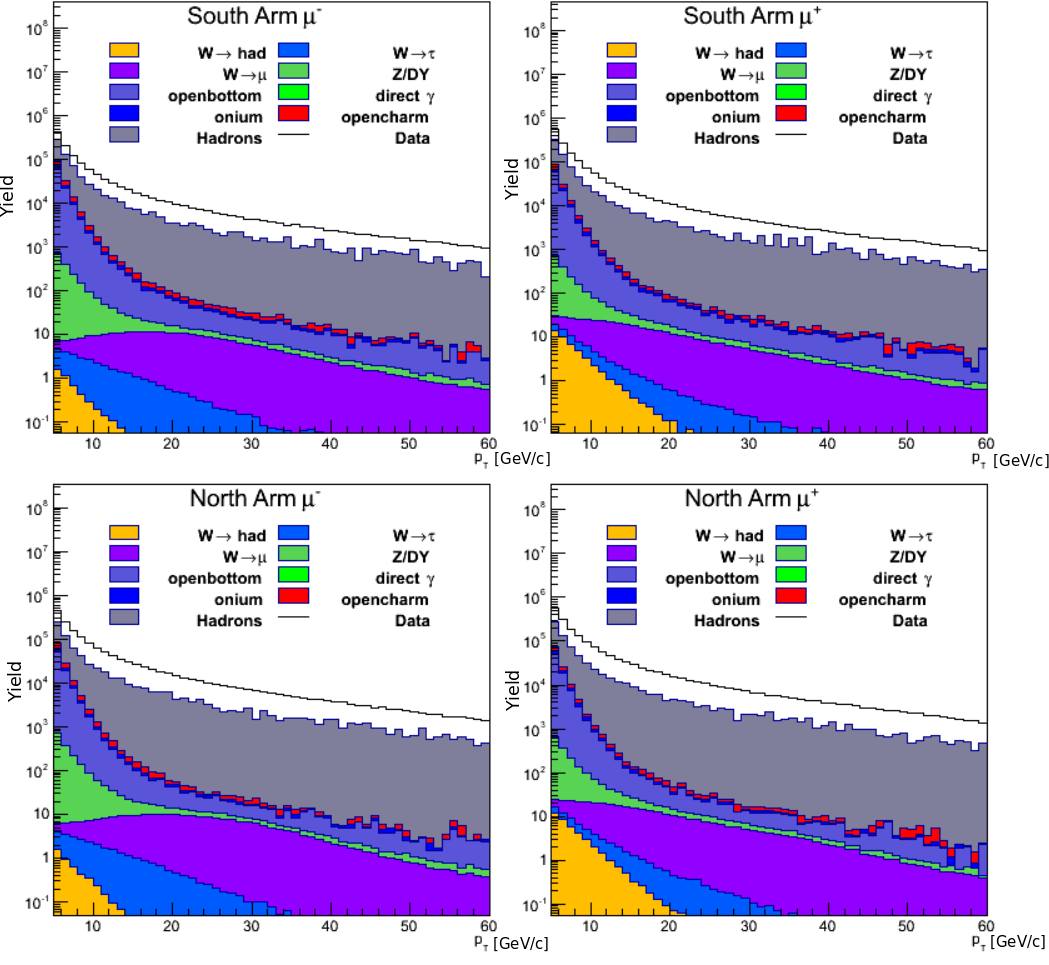
\includegraphics[width=\linewidth]{./figures/stacked_xsec.png}
  \caption{
    Shown: stacked cross-sections of all simulated processes as a
    function of $p_T$. All data shown has been created from the PISA+PYTHIA
    framework. Top Left: South $\mu-$, Top Right: South $\mu+$, Bottom Left:
    North $\mu+$, Bottom Right: North $\mu-$~\cite{Seidl2014a}
  }
  \label{fig:stacked_xsec_sim}
\end{figure}

\clearpage


\section{$W_{ness}$: Likelihood Event Tagging}
\label{sec:likelihood}

Recalling that the dataset into is already split into three main contributions:
hadronic background, real muon background, and W-Signal, the next task is to 
formulate a means to separate signal from background.

Previous analyses have attempted to separate the muon spectrum into $p_T$ bins,
to estimate the composition, however, because the $W\rightarrow\mu$ signal is so
small in the forward kinematic regime, these methods are not viable, as
there is no `visible' cutoff in the spectrum associated with a invariant mass
peak at half the mass of the $W$ Boson.

High momentum $\mu$ tracks are straight, with less bending then other $\mu$
tracks. The kinematic variables describing track reconstruction have
characterisitcally narrow distributions for our signal muons.

One can think of the study of the data set in terms of a classification problem.
Bayes Theorem is at the foundation of a robust classification technique, known
Naive Bayes. Using this technique to classify a data requres that one has a
sample of labeled testing data to construct a model which can classify data into
two or more classes. Care must be taken not over-train the classifier, or
attempt to classify data which has been used in the subset of data to train the
classifier. An example of over-training might be a case where one customizes the
model by providing training data which is not representative of the real
variation in the true data set, which artifically inflates the model's
accuracy when used on training data.

In our case, we have simulations which serve as the training data, guaranteeing
that there will be no overlap between the physical data produced, and the data
used to train the classifier. Thus, we implement a Naive Bayes Classifier (also
known as Likelihood Selection) to label our data with two classes. Rather than
labeling data with a binary classification, however, we opt to label the data
with its likelihood, a posterior probability which tells us if a value is more
or less likely to come from a $W$ Boson.

\subsection{Naive Bayes Classification}

Although there are many techniques available for classifying a collection of
variables (a feature set) into categories. Naive Bayes classification is an
excellent candidate for classification. Naive Bayes can be useful in cases where
we have meaningful classification categories which can be applied to feature
sets. The feature sets must not be correlated, since this can lead to over
training.  Naive Bayes is a robust, fast, scalable machine learning technique.
Originally used for classification of text documents, Naive Bayes is also able
to handle numeric features whose distributions are known~\cite{Collins2013}.

In this analysis, consider our track reconstruction variables as the `feature
set', and the classification of `signal' or `background' as the label.

In order to obtain the best performance from the classifier, without
over-training, one must ensure that the variables used to determine a class are
maximally uncorrelated. The variables which match this criteria are: DG0, DDG0,
$\chi^2$, $fvtx$ variables, Rpc1DCA, Rpc3DCA, DCA$_r$, and DCA$_z$. The linear
correlations between these variables are shown for both the data, and the
simulated W-Signal in Figure~\ref{fig:kinematic_var_correlations}.

\begin{figure}[H]
	\centering
	\begin{subfigure}[t]{0.5\textwidth}
		\centering
		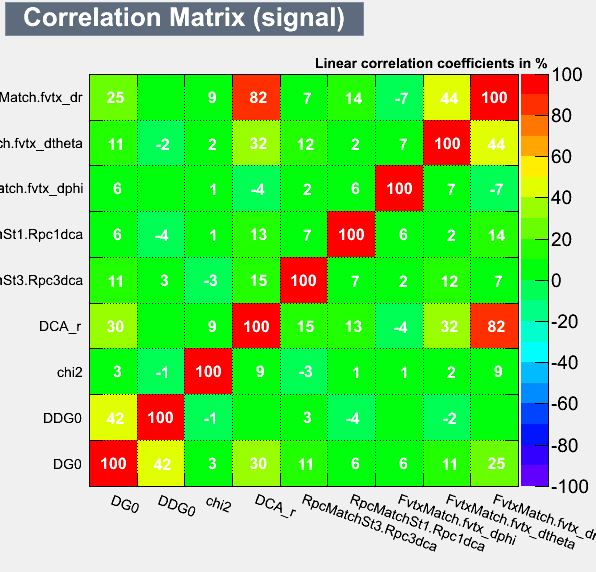
\includegraphics[width=0.95\linewidth]{./figures/CorrelationMatrix_Signal.png}
		\caption{
      Simulated $W$ Boson $\mu$ events
    }
		\label{fig:corr_mat_sig}
	\end{subfigure}%
  \begin{subfigure}[t]{0.5\textwidth}
		\centering
		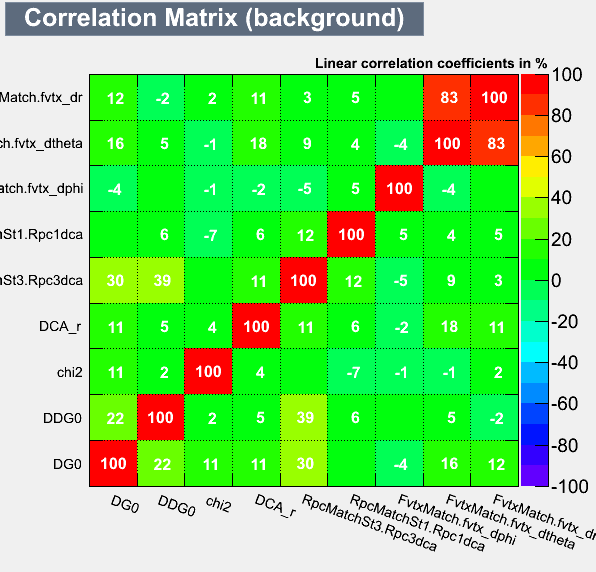
\includegraphics[width=0.95\linewidth]{./figures/CorrelationMatrix_Background.png}
		\caption{
      Real data proxy for hadronic background
    }
		\label{fig:corr_mat_bkg}
	\end{subfigure}
	\caption{ 
    In panel (a) Correlations are shown between kinematic variables, produced
    from the signal simulation. In panel (b) correlations are shown for the real
    data proxy for hadronic background. Variables that are correlated are
    combined in two dimensional probability distribution functions, i.e. DG0 and
    DDG0 and DCA$_r$ and $\chi^2$.
    }
	\label{fig:kinematic_var_correlations}
\end{figure}

As one can see from Figure~\ref{fig:kinematic_var_correlations}, DG0 and DDG0
are slightly correlated, as are $\chi^2$ and DCA$_r$. A Naive Bayes classifier
may be constructed from the core of the familiar Bayes Theorem from probability
and statistics. In our case, we understand Naive Bayes as a conditional
probability. Concretely, we consider a vector of features (i.e.  our
discriminating kinematic variables):

\begin{equation}
	\label{eq:feature_vector}
\mathbf{x} = (x_1, \dots, x_n)
\end{equation}

{\noindent}and assume independence between each feature $x_n$. We then define the
probability of a given classification, $C_k$ (i.e. signal or background) given a
set of features $x_n$ (i.e. DCA$_r$, $\chi^2$ ...):

\begin{equation}
	\label{eq:cond_probabilty}
  \mathcal{P}(C_k \vert x_1, \dots, x_n)
\end{equation}

{\noindent}This conditional probability is defined in terms of Bayes Theorem:

\begin{equation}
	\label{eq:bayes_theorm}
  \mathcal{P}(C_k \vert \mathbf{x}) = \frac{\mathcal{P}(C_k) \
  \mathcal{P}(\mathbf{x} \vert C_k)}{\mathcal{P}(\mathbf{x})}
\end{equation}

{\noindent}The terms here are defined as:
\begin{itemize}
  \item $\mathcal{P}(C_k)\rightarrow$ prior probability
	\item $\mathcal{P}(\mathbf{x} \vert C_k)\rightarrow$ likelihood
	\item $\mathcal{P}(\mathbf{x})\rightarrow$ overall probabiltiy
\end{itemize}

The probabilities described here are realized through constructing probability
density functions from the data and simulations. The constraints for choosing
PDFs to use represent the two lables are: (1) PDFs must be able to be
meaningfully normalized, (2) PDFs associated with each label should have a
unique enough shape to differentiate between either label, and (3) the PDFs
should be uncorrellated.
 

The likelihood ratio is constructed using the posterior probability
for each classification, which is defined as $W_{ness}$:
\begin{align*}
  \lambda_{sig} &= \prod_{k}\mathcal{P}(\mu_{sig}\vert C_k)\\
  \lambda_{bak} &= \prod_{k}\mathcal{P}(\mu_{bak}\vert C_k)\\
  W_{ness} &= { 
    {\lambda_{sig}}
    \over 
    {\lambda_{sig}+\lambda_{bak}} 
  }\label{eq:wness_calculation}
\end{align*}

{\noindent}Where $\lambda_{sig}$ and $\lambda_{bak}$ represent the total
likelihoods that a given track is either signal, or background, constructed from
the product of likelihoods calculated from each probability density function.

In order to construct probability distribution functions to use in this
classification, one must select samples of labeled data representing each
classification. The recorded data is used as a proxy the `background' labeled
data set, and the simulation of the $W$ boson decay is the `signal' labeled data
set. The $W$ Boson signal at this stage of the analysis does not meaningfully
change the shape of the PDFs extracted from the data. Even after the Basic Cut,
the number of $W$ Boson decay events is small relative to the hadronic and muon
background (less than one part in 1000). The $W$ Boson production cross section
is precisely known--since the luminosity delivered to PHENIX is also known, the
$W$ Boson yield may be trivially estimated.

Not all recorded events contain valid tracking information for all tracks. For
example, consider a muon track which was recorded due to a minimum bias trigger.
When any trigger causes data to be recorded, there is no guarantee that all
subsystems have been triggered, but all subsystems flush the data in their
buffers to the archival data stream. This is not an error, each detector
subsystem has an associated efficiency and acceptance.  For example, with our
example track, perhaps the physical process related to triggering a detector
simply didn't occur. One may correct account for all this when constructing
PDFs.  A selection process is superimposed such PDFs are constructed only from
events (simulated or otherwise) containing valid data. Similarly, the selection
process must also be preserved when looking up what PDFs to ultimately use in
calculating the likelihood of an event being generated from a signal process.
This process is represented in Figure~\ref{fig:pdf_selection_tree}.

\begin{figure}[ht]
  \centering
  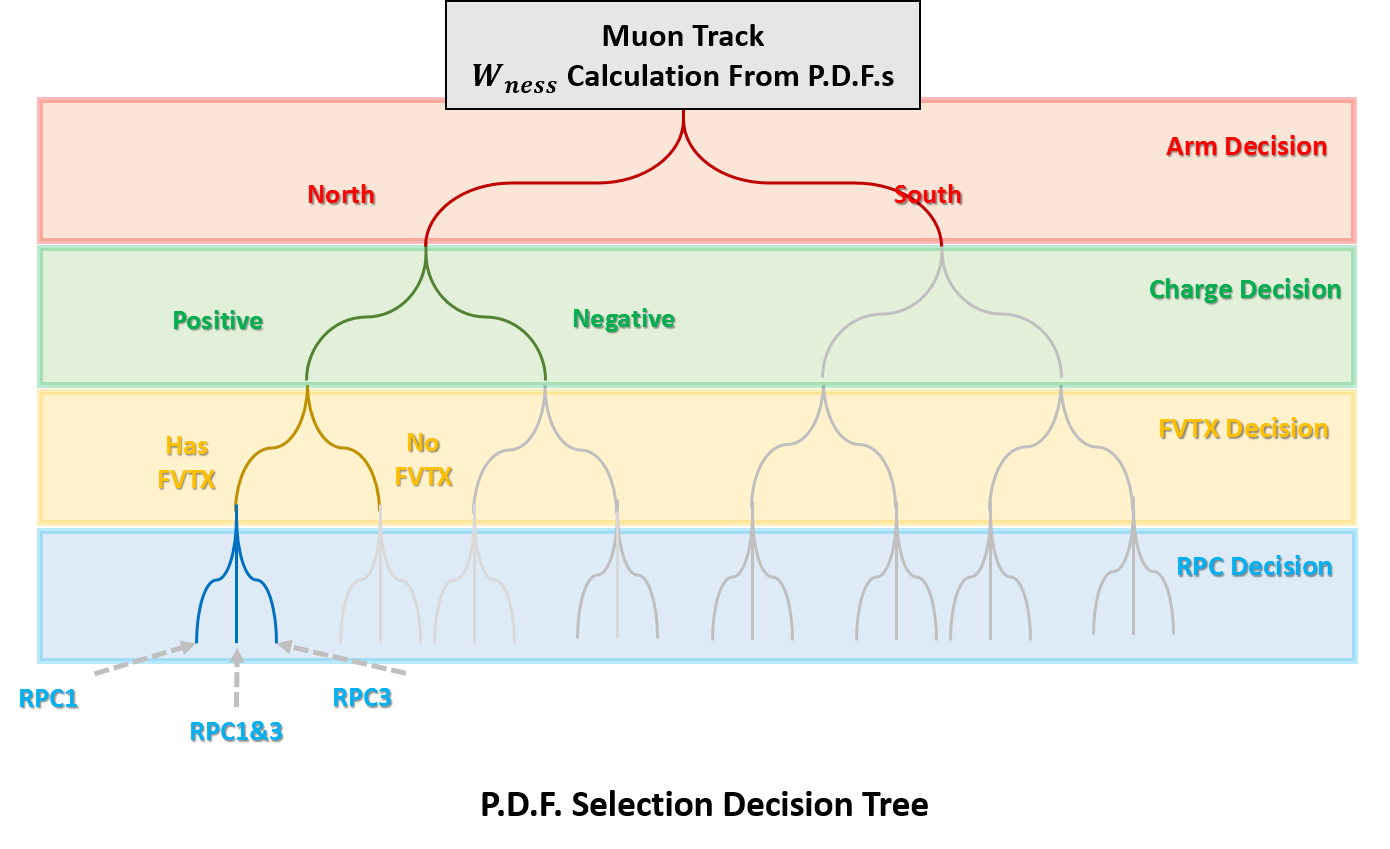
\includegraphics[width=\linewidth,trim=4 4 4 4,clip]{./figures/pdf_selection_tree.png}
  \caption{
    A cartoon of the decision tree to determine the PDF cocktail to use for
    quantifying the $W_{ness}$ of a given track. The track's properties are used
    to traverse the tree, and select the cocktail contents.
  }
  \label{fig:pdf_selection_tree}
\end{figure}

Finally, once all PDFs have been constructed, following the selection process
shown in Figure~\ref{fig:pdf_selection_tree}, one may loop over the simulated
data set, and the recorded data set, and perform the likelihood calculation for
each muon track (Equation~\ref{eq:wness_calculation}). The value of
"$W_{ness}$" is stored for every track in the simulation and data as an
engineered feature to be used in cuts.

In figures~\ref{fig:pdf_rpc3dca}-\ref{fig:pdf_DG0}, we can see the various
distributions which are used to create probability distribution functions. In
the figures, we represent the product of all probability functions which are
used to tag an event as $\lambda$ such that 
$\lambda = \Pi_{k} \mathcal{P}(\mu \vert C_k)$.

\begin{figure}
  \centering
  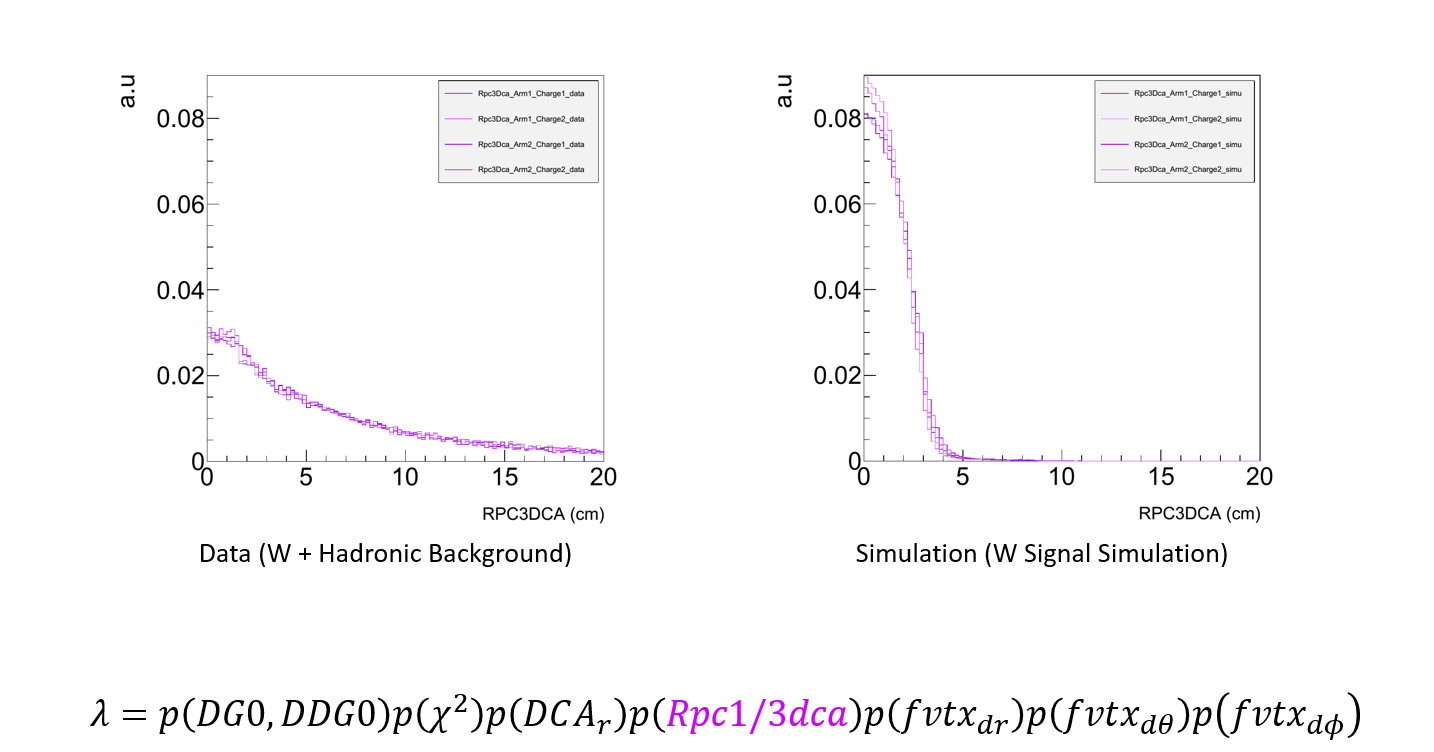
\includegraphics[width=\linewidth,trim=4 4 4 4,clip]{./figures/pdf_rpc3dca.png}
  \caption{
    Left: the distribution of Rpc3dca for each arm and charge, produced from the
    PHENIX data set, after the basic cut. Right: the same distributions from a
    simulation of the W-Signal.
  }
  \label{fig:pdf_rpc3dca}
\end{figure}

\begin{figure}
  \centering
  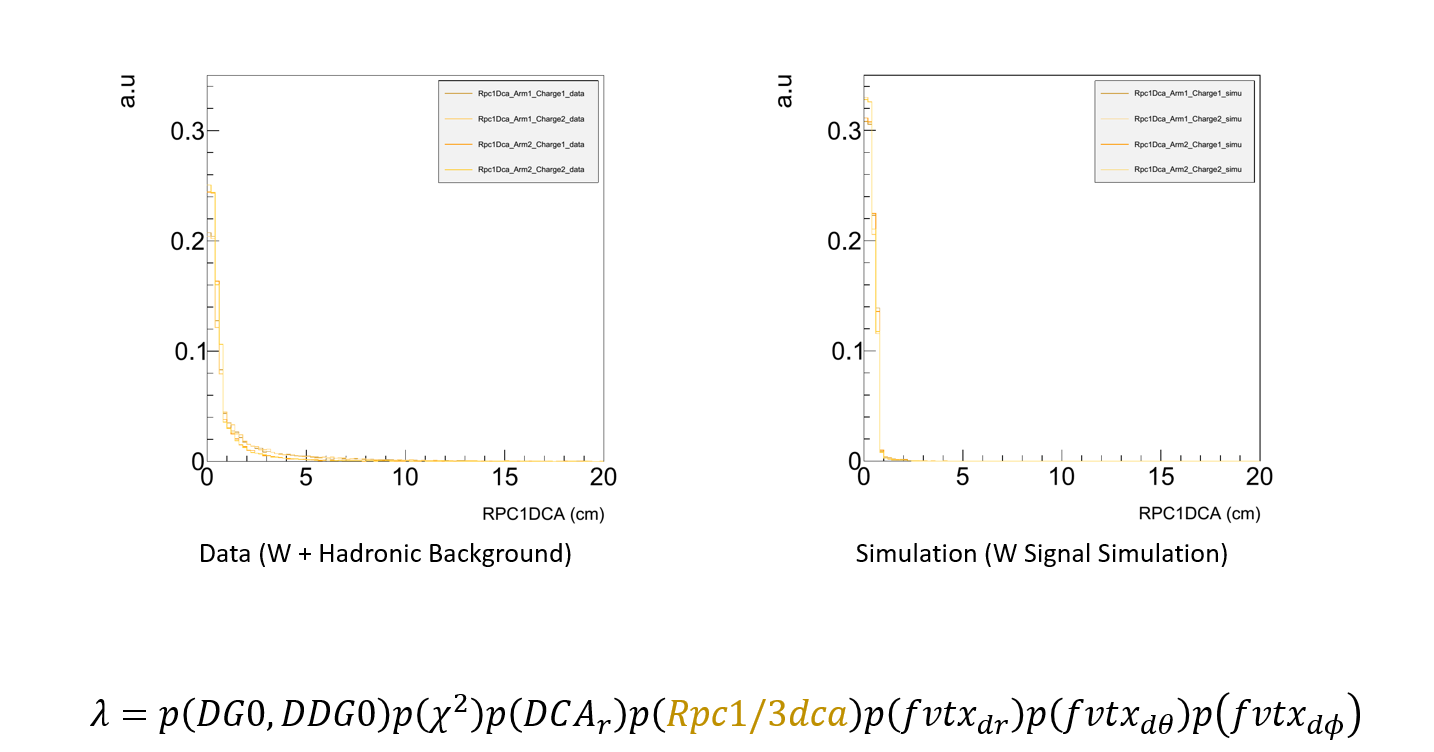
\includegraphics[width=\linewidth,trim=4 4 4 4,clip]{./figures/pdf_rpc1dca.png}
  \caption{
    Left: the distribution of Rpc1dca for each arm and charge, produced from the
    PHENIX data set, after the basic cut. Right: the same distributions from a
    simulation of the W-Signal.
  }
  \label{fig:pdf_rpc1dca}
\end{figure}

\begin{figure}
  \centering
  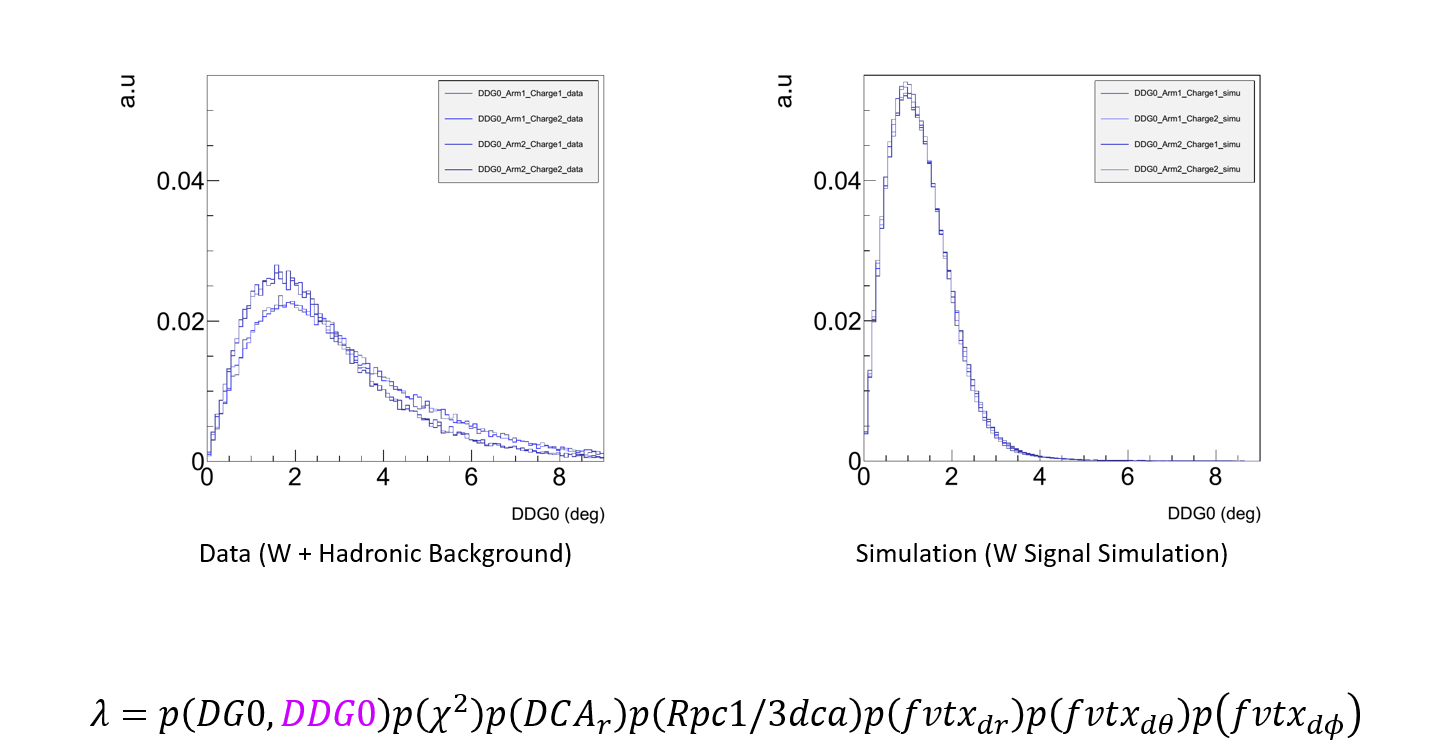
\includegraphics[width=\linewidth,trim=4 4 4 4,clip]{./figures/pdf_DDG0.png}
  \caption{
    Left: the distribution of DDG0 for each arm and charge, produced from the
    PHENIX data set, after the basic cut. Right: the same distributions from a
    simulation of the W-Signal.
  }
  \label{fig:pdf_DDG0}
\end{figure}

\begin{figure}
  \centering
  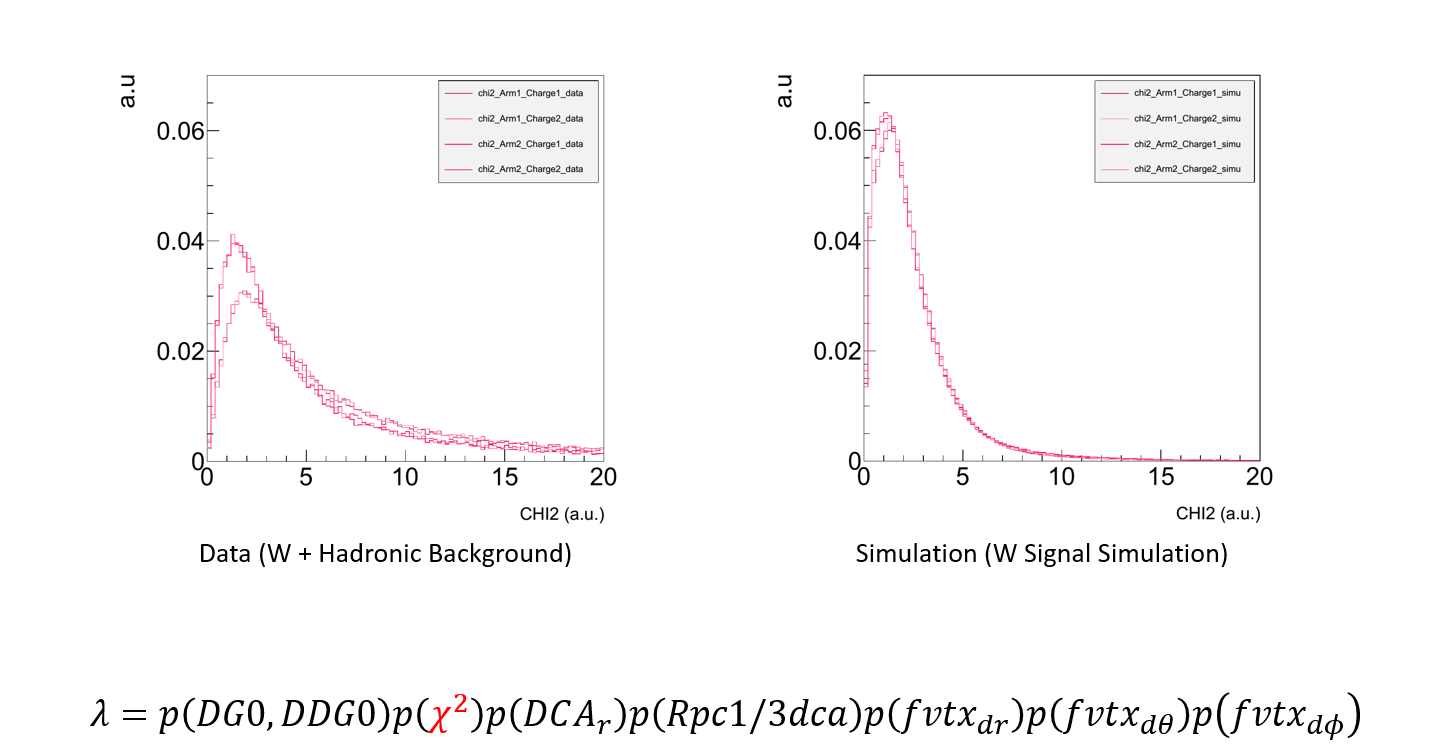
\includegraphics[width=\linewidth,trim=4 4 4 4,clip]{./figures/pdf_chi2.png}
  \caption{
    Left: the distribution of $\chi^2$ for each arm and charge, produced from the
    PHENIX data set, after the basic cut. Right: the same distributions from a
    simulation of the W-Signal.
  }
  \label{fig:pdf_chi2}
\end{figure}

\begin{figure}
  \centering
  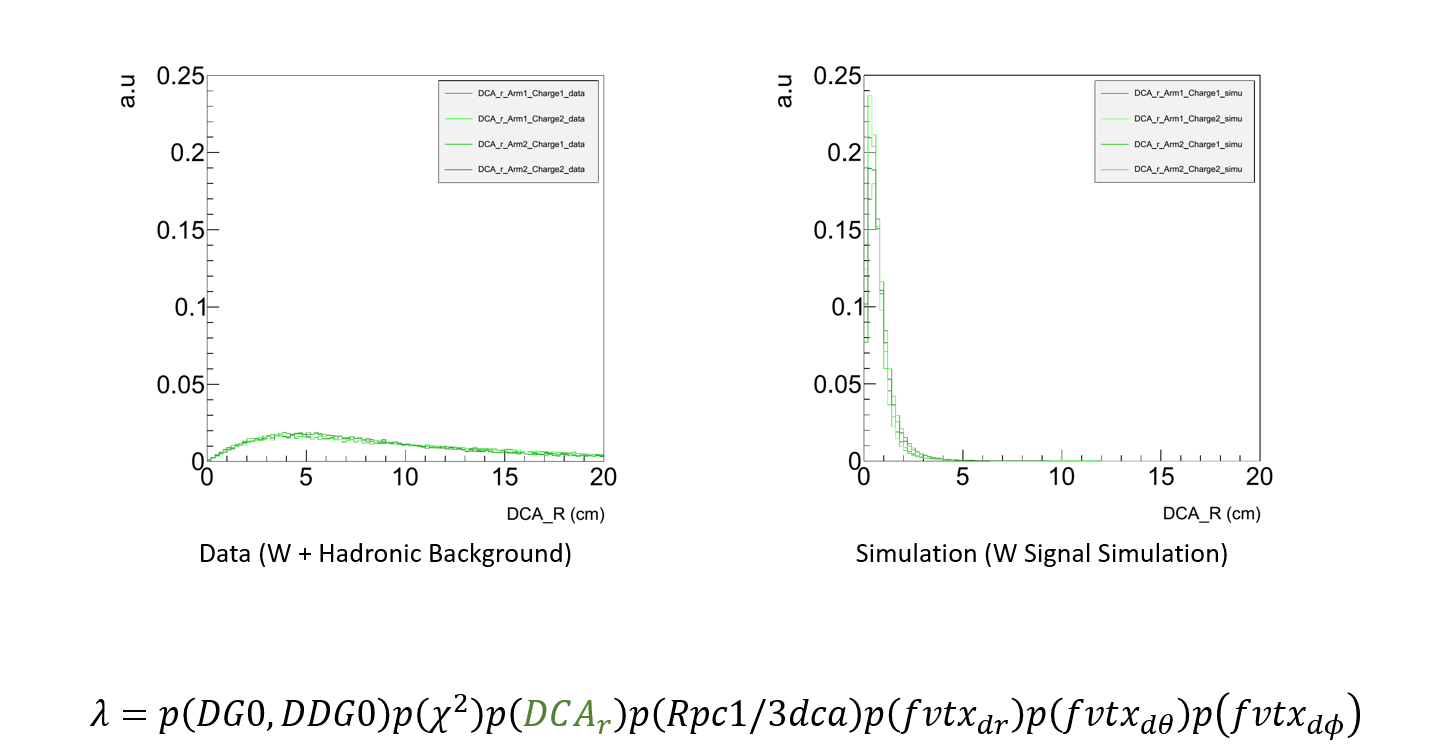
\includegraphics[width=\linewidth,trim=4 4 4 4,clip]{./figures/pdf_dcar.png}
  \caption{
    Left: the distribution of DCA$_r$ for each arm and charge, produced from the
    PHENIX data set, after the basic cut. Right: the same distributions from a
    simulation of the W-Signal.
  }
  \label{fig:pdf_dcar}
\end{figure}

\begin{figure}
  \centering
  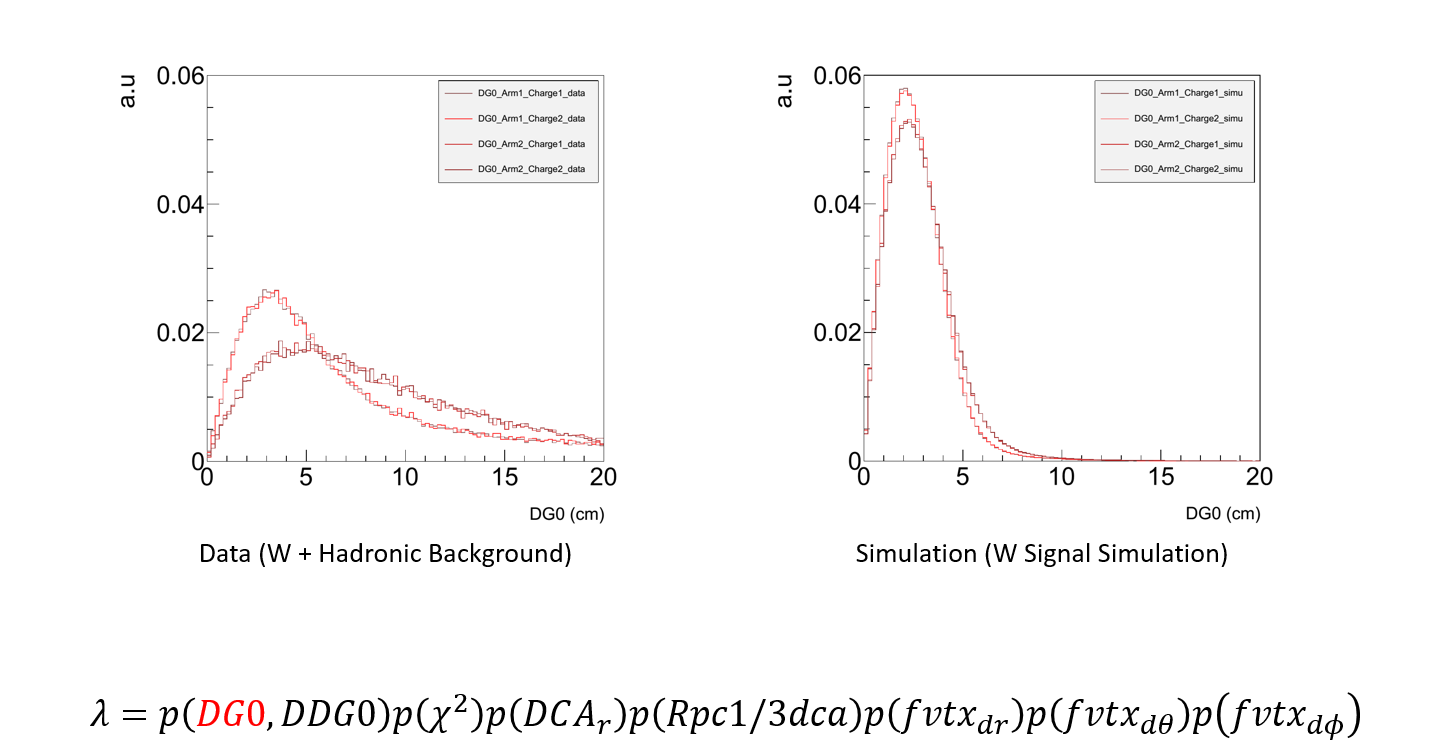
\includegraphics[width=\linewidth,trim=4 4 4 4,clip]{./figures/pdf_DG0.png}
  \caption{
    Left: the distribution of DG0 for each arm and charge, produced from the
    PHENIX data set, after the basic cut. Right: the same distributions from a
    simulation of the W-Signal.
  }
  \label{fig:pdf_DG0}
\end{figure}

Now that we have a complete set of probability density functions which predict
the likelihood that a given track is a W-genic muon or not, we can loop over the
real physics data set, and use our likelihood calculation strategy to label
every muon track with a $W_{ness}$. We may also tag our simulated data set with
$W_{ness}$. The distributions are shown in
Figure~\ref{fig:wness_distribution}.

\begin{figure}
  \centering
  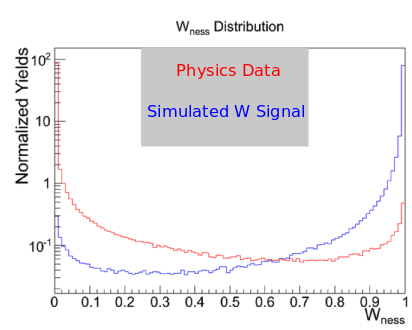
\includegraphics[width=0.7\linewidth]{./figures/wness_sig_bak.png}
  \caption{
    After $W_{ness}$ tagging, we can visualize the classification of signal from
    background by comparing the distribution of $W_{ness}$ in
    \textcolor{red}{physics data}, and the \textcolor{blue}{simulated data}
    data. Note that the vertical is plotted on a log scale. The two
    distributions have been normalized prior to plotting. Additionally, the
    physics data is used as a proxy for the hadronic background, from $W_{ness}
    < 0.95$.
  }
  \label{fig:wness_distribution}
\end{figure}

As we can see from Figure~\ref{fig:wness_distribution}, most of the simulated
data falls in the high $W_{ness}$ range while most of the physics data falls in
the low $W_{ness}$ range. The goal of the likelihood analysis is to tag the data
with $W_{ness}$ such that we can apply a cut on the data based on the
parameter's value. We wish to apply the cut in a way that minimally removes any
signal, and we may calculate the efficiency of this cut, summarized in
Figure~\ref{fig:wness_cut_efficiency}.

\begin{figure}
  \centering
  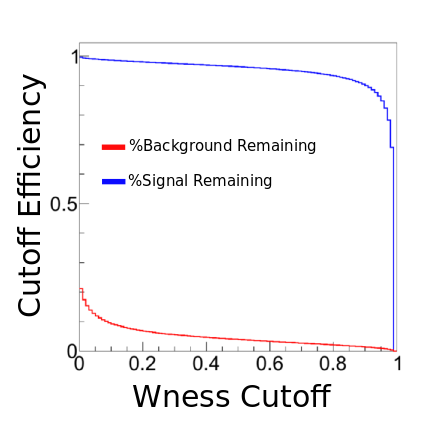
\includegraphics[width=0.7\linewidth]{./figures/wness_cut_efficiency.png}
  \caption{
    We look at the fraction of signal and background remaining in the total data
    set as we make successively higher cuts in $W_{ness}$. At the turning point
    of the blue distribution. We know this, because the $W$ Boson production
    cross section is accurately known, and we can measure the Luminosity
    delivered to PHENIX. 
  }
  \label{fig:wness_cut_efficiency}
\end{figure}

As we make successive cuts in $W_{ness}$, we find that the optimum cutoff is at
$W_{ness} < 0.95$. We can throw out all data below this threshold, and
maintain a good portion of our signal data.

Note that now with this reduced data set, we could simply assume that all
remaining data is signal, and calculate an asymmetry, however, there is clearly
still a lot of background present. Any background that is still present will
dilute our main observable, $A_L$. Therefore, we employ the unbinned maximum
likelihood fit to a three dimensional data set, composed of $W_{ness}$, $\eta$,
and $dw_{23}$.

\clearpage
\section{Extended Unbinned Maximum Likelihood Selection: The Signal to
Background Ratio}
\label{sec:sbr}

The goal of the Extended Unbinned Maximum Likelihood Fit (EULMF) is to calculate
the signal to background ratio, so that we can calculate $A_L$ and correct for
the dilution from the background. The EULMF is another statistical method which
relies on creating Probability Density Functions to represent the likelihood of
given track to originate from a known source. However, at this stage in the
analysis, we are interested in subdividing the background data set into
contributions from the Hadronic Background and the Muon Background. We form our
PDFs for the Muon Background by weighting the various individual muon
processes and adding them together such that the relative frequencies of each
process are comparable to the composition of the real physics data set. In broad
strokes, we want to generate PDFs in the dimension of $\eta$ and $dw_{23}$ for
Hadronic Background, Muon Background, and W-Signal distributions. However, since
we will be applying this fit to a data set where we have applied a $W_{ness}$
cut, we must be very careful to not over or under-fit the hadronic background. 

In order to accomplish this, we parameterize the data set as a 2D function in
$dw_{23}$ and $W_{ness}$. We then fit this distribution, generated from the
physics data, with a parameterization, over the nominal hadronic background
dominated region from $0 < W_{ness} < 0.95$. We then extrapolate the shape
of $dw_{23}$ into the high $W_{ness} > 0.95$ region, hereafter referred to as
the `signal region', with $W_{ness} < 0.95$ referred to as the `background
region'.

Similarly to any analysis which uses probability density functions, the PDFs
representing $\eta$ and $dw_{23}$ must be uncorrelated so as to not over-fit
the data.

The purpose of the EULMF is to essentially scale the PDFs for each arm and
charge for $\eta$ and $dw_{23}$ so as to obtain yields for W-genic muons, Muon
Background muons, and hadronic background fake muons.

To use this method, we must construct the likelihood function
(Equation~\ref{eq:likelihood_function}) and maximize it. We write down the
likelihood function in as a product of the individual likelihoods:


An unbinned maximum likelihood fit can then be performed to extract the number
of events for each process: $n_{sig},\,n_\mu,\, n_{had}$. The likelihood
function is defined accounting for a Poisson  distribution of the events $x_i$:

\begin{equation} 
  \mathcal{L}(\theta|X) 
  \equiv
  \frac{n^N e^{-n}}{N!} \prod_{x_i \in X}^N
  \sum_c \frac{n_c}{n} p_c (x_i), \
  ;{\rm with}\, 
  n=\sum_c n_c 
  \label{eq:likelihood_function}
\end{equation} 

where $X$ is the sample of $N$ total events $x_i = (\eta_i,dw_{23i})$, and
$\theta$ gives the parameters of the fit $\theta = (n_{sig},\,n_\mu,\,
n_{had})$.  $c$ is an index running over the three data types (muon background,
hadronic background, w-signal). To reduce the number of parameters, we fixed the
number of muon background events $n_\mu$ to the expected yield according to the
cross section of muon background processes, and then we extracted the remaining
parameters $(n_{sig},\, n_{had})$ by minimizing the
$-\log(\mathcal{L}(\theta|X))$.  With Run 13 data we have enough statistics to
divide the data sample in three $\eta$ region: $1.10 < \eta < 1.40$, $1.40 <
\eta < 1.80$ and $1.80 < \eta < 2.60$. 

\subsection{Hadronic Background PDFs}

The main analysis challenge for the EULMF is obtaining an adequate description
of the $dw_{23}$ and $\eta$ distributions for the hadronic background. They are
shown, along with the $W_{ness}$ distribution for the data, for the background
region, in Figure~\ref{fig:dw23_eta_wness_dat}, and the simulated W-genic data
in Figure~\ref{fig:dw23_eta_wness_sim}.

\begin{figure}
  \centering
  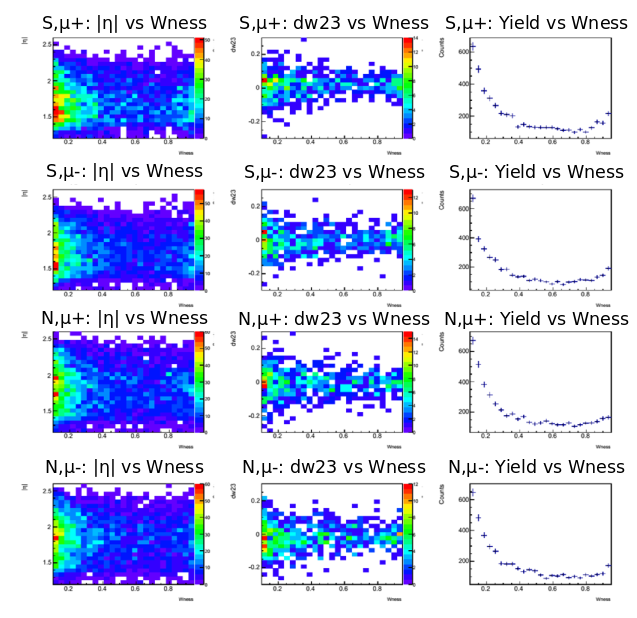
\includegraphics[width=\linewidth]{./figures/dw23_vs_wness_data.png}
  \caption{
    The first column of plots is $\eta$ plotted as a function of $W_{ness}$
    where we see a 2D histogram of the even distribution. The middle column is
    $dw_{23}$ as a function of $W_{ness}$, and the right column is a simple
    histogram of $W_{ness}$. The rows all correspond to the same arm and charge.
    From top to bottom: North, $\mu+$, North $\mu-$, South $\mu+$, North $\mu-$.
    Distributions shown here are all from the physics data set.
  }
  \label{fig:dw23_eta_wness_dat}
\end{figure}

\begin{figure}
  \centering
  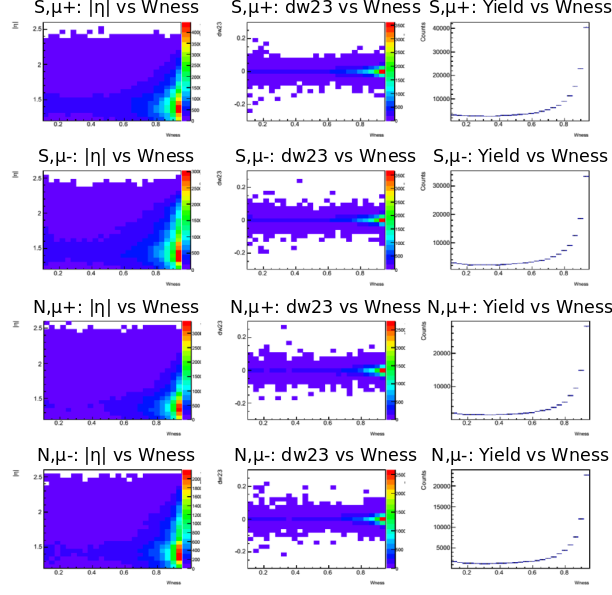
\includegraphics[width=\linewidth]{./figures/dw23_vs_wness_simulation.png}
  \caption{
    The first column of plots is $\eta$ plotted as a function of $W_{ness}$
    where we see a 2D histogram of the even distribution. The middle column is
    $dw_{23}$ as a function of $W_{ness}$, and the right column is a simple
    histogram of $W_{ness}$. The rows all correspond to the same arm and charge.
    From top to bottom: North, $\mu+$, North $\mu-$, South $\mu+$, North $\mu-$.
    Distributions shown here are all from simulated W-genic data set.
  }
  \label{fig:dw23_eta_wness_sim}
\end{figure}

Two features to note from Figure~\ref{fig:dw23_eta_wness_dat} and
Figure~\ref{fig:dw23_eta_wness_sim} is that the distribution for $dw_{23}$
should be expected to be quite narrow for W-genic events, whereas $\eta$ is more
broad. We have good statistic for $\eta$ over all orders of magnitude, so we can
directly construct PDFs for this variable from a binned dataset. However, with
$dw_{23}$ we need to be more careful, as this variable will offer us the
analyzing power.

We create a model for $dw_{23}$, to fully parameterize the event distribution
when viewed as a function of $dw_{23}$ vs $W_{ness}$. We model this by assuming
that the $dw_{23}$ vs $W_{ness}$ distribution can be separated into two parts:

\begin{equation}
  F(W_{ness},dw_{23}) = f(W_{ness})\times g(W_{ness},dw_{23}) 
  \label{eq:dw23_final_parameterization}
\end{equation}

$f(W_{ness})$ is modeled simply as a fourth-degree polynomial (the third column)
of Figures~\ref{fig:dw23_eta_wness_dat} and \ref{fig:dw23_eta_wness_sim}. The
polynomial fit is summarized in Equation~\ref{eq:wness_pol4} and
Figure~\ref{fig:wness_pol4}:

\begin{equation} \label{eq:wness_pol4}
  f(W_{ness}) = 
  P_8 + P_9 W_{ness} + 
  P_{10} {W_{ness}}^2 +
  P_{11} + {W_{ness}}^3 +
  P_{12} + {W_{ness}}^4
\end{equation}

\begin{figure}
  \centering
  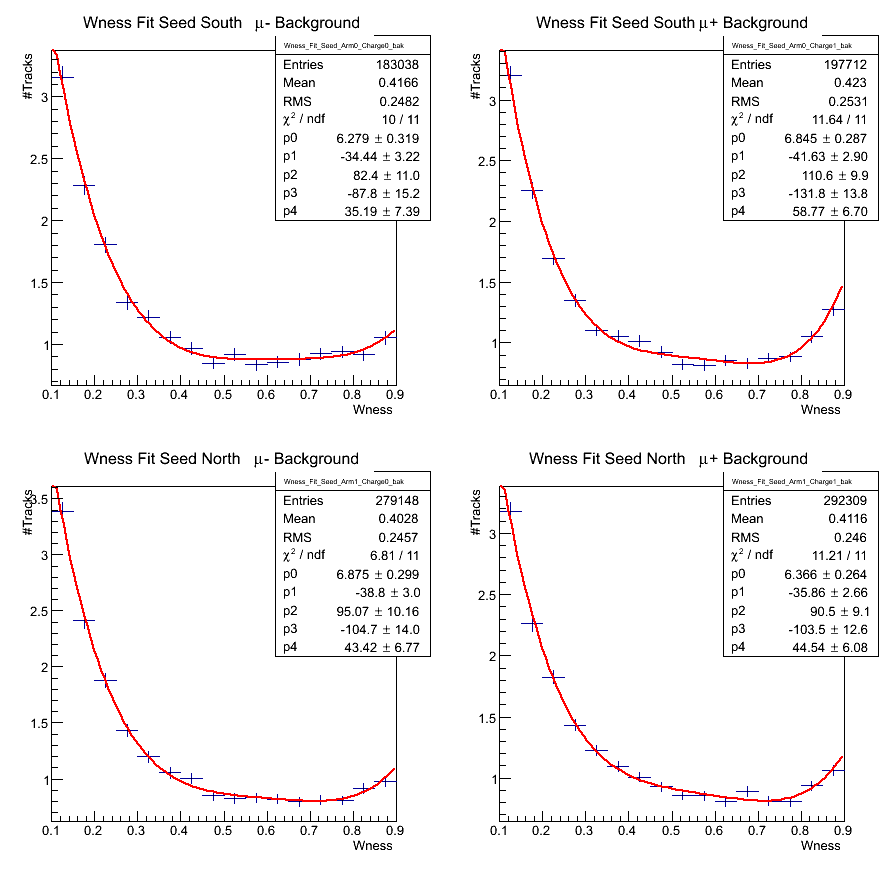
\includegraphics[width=0.7\linewidth]{./figures/c_WnessFit1D.png}
  \caption{
    A summary of the fourth degree polynomial fit (Equation~\ref{eq:wness_pol4})
    to the $W_{ness}$ distribution from the physics dataset in the background
    region.
  }

  \label{fig:wness_pol4}
\end{figure}

We then model the other element of the distribution $g(W_{ness},dw_{23}$ as a
co-axial double Gaussian. We allow the Parameters of the co-axial double
Gaussian to vary linearly with $W_{ness}$, as seen below:

\begin{align}\label{eq_dw23_equations}
  \sigma_1 &= P_1 + P_3 \times W_{ness} &  C_g &= P_6 + P_7 \times W_{ness} \\
  \sigma_2 &= P_4 + P_5 \times W_{ness} &  \mu &= P_0 + P_1 \times W_{ness}
\end{align}

\begin{equation}
  g(W_{ness},dw_{23}) = C_w \times 
  \left(
    \left( 
      { {1}\over{\sqrt{2\pi}\sigma_1+C_g\sqrt{2\pi}\sigma_2} }
    \right) 
    \times
    \left(
      e^{{{1}\over{2}}{\left({dw_{23-\mu}}\over{\sigma_1}\right)^2}}
        +C_ge^{{{1}\over{2}}{\left({dw_{23-\mu}}\over{\sigma_2}\right)^2}} 
    \right) 
  \right)
  \label{eq:dw23_parameterization}
\end{equation}

We seed these linearized parameters by taking slices of $dw_{23}$ in $W_{ness}$
and then fitting this slice with a co-axial double Gaussian. The parameters of
the results of these fits are then plotted against the value of the $W_{ness}$
slice, and fit with a line. These parameters are then used to seed the fit of
Equation~\ref{eq:dw23_final_parameterization} to the physics data set. Fits to
the individual slices of $dw_{23}$ are summarized in
Figure~\ref{fig:dw23_slice_fits}. The results of the co-axial double Gaussian
parameters as functions of $W_{ness}$ slice are shown in
Figure~\ref{fig:coax_params_vs_wness}.

\begin{figure}
  \centering
  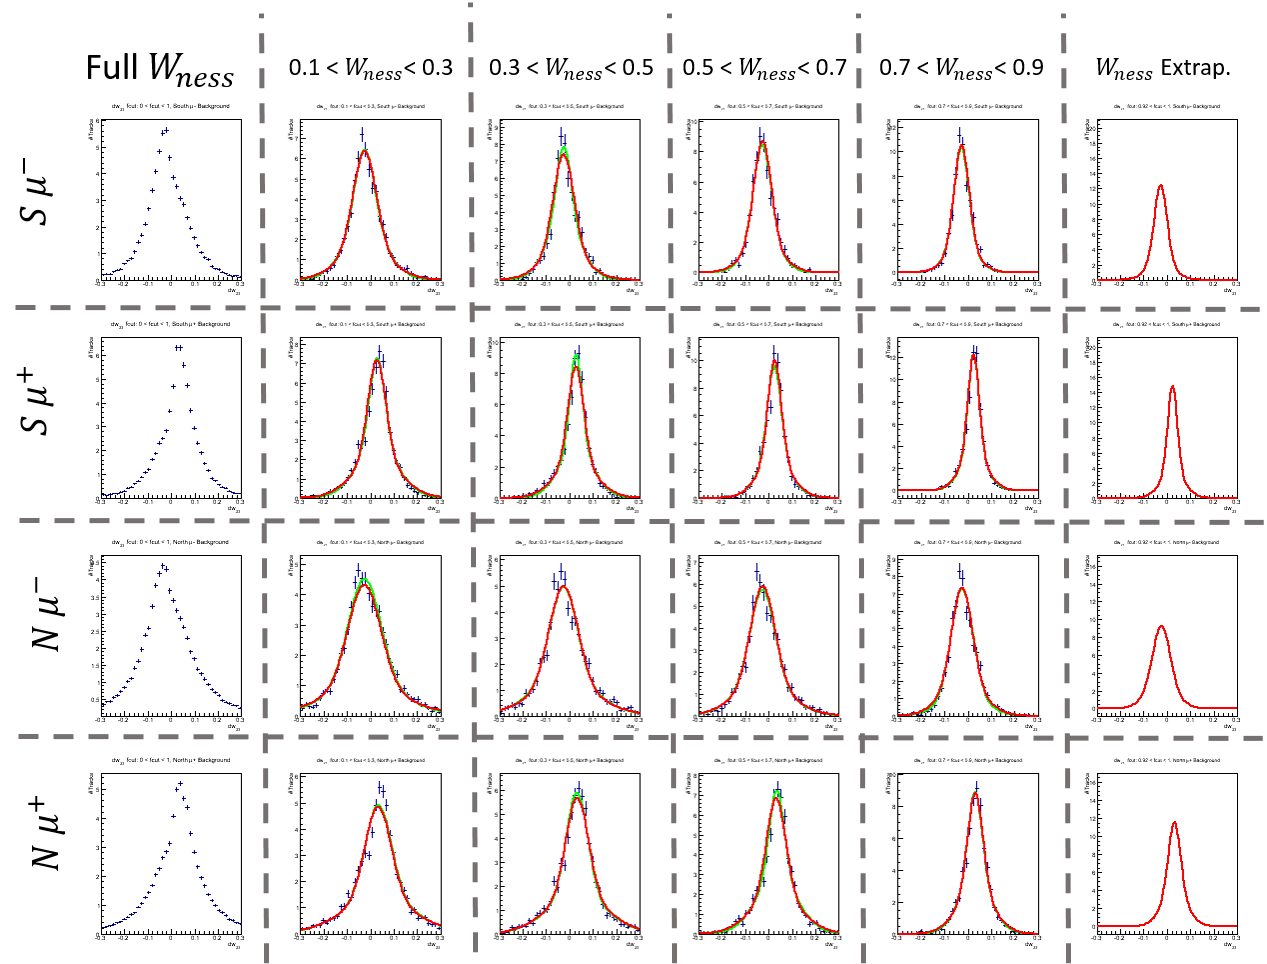
\includegraphics[width=\linewidth]{./figures/dw23_extrap_bins.png}
  \caption{
    From left to right the columns are: $dw_{23}$ for the full $W_{ness}$ range,
    $0.1 < W_{ness} < 0.3$, $0.3 < W_{ness} < 0.7$, $0.3 < W_{ness} < 0.7$, 
    $0.7 < W_{ness} < 0.9$, and finally the extrapolated shape for $W_{ness} >
    0.95$. In red, we see the 1D projection of the 2D distribution to the slice.
    This overlays a green curve, which is a fit done independently to a slice.
    The rows are labeled with the Arm and charge corresponding to the subdivided
    dataset. As you can see, the matching is often exact, between green and red
    curves. As the final column is the extrapolation, there is no slice-fit.
  }
  \label{fig:dw23_slice_fits}
\end{figure}

\begin{figure}
  \centering
  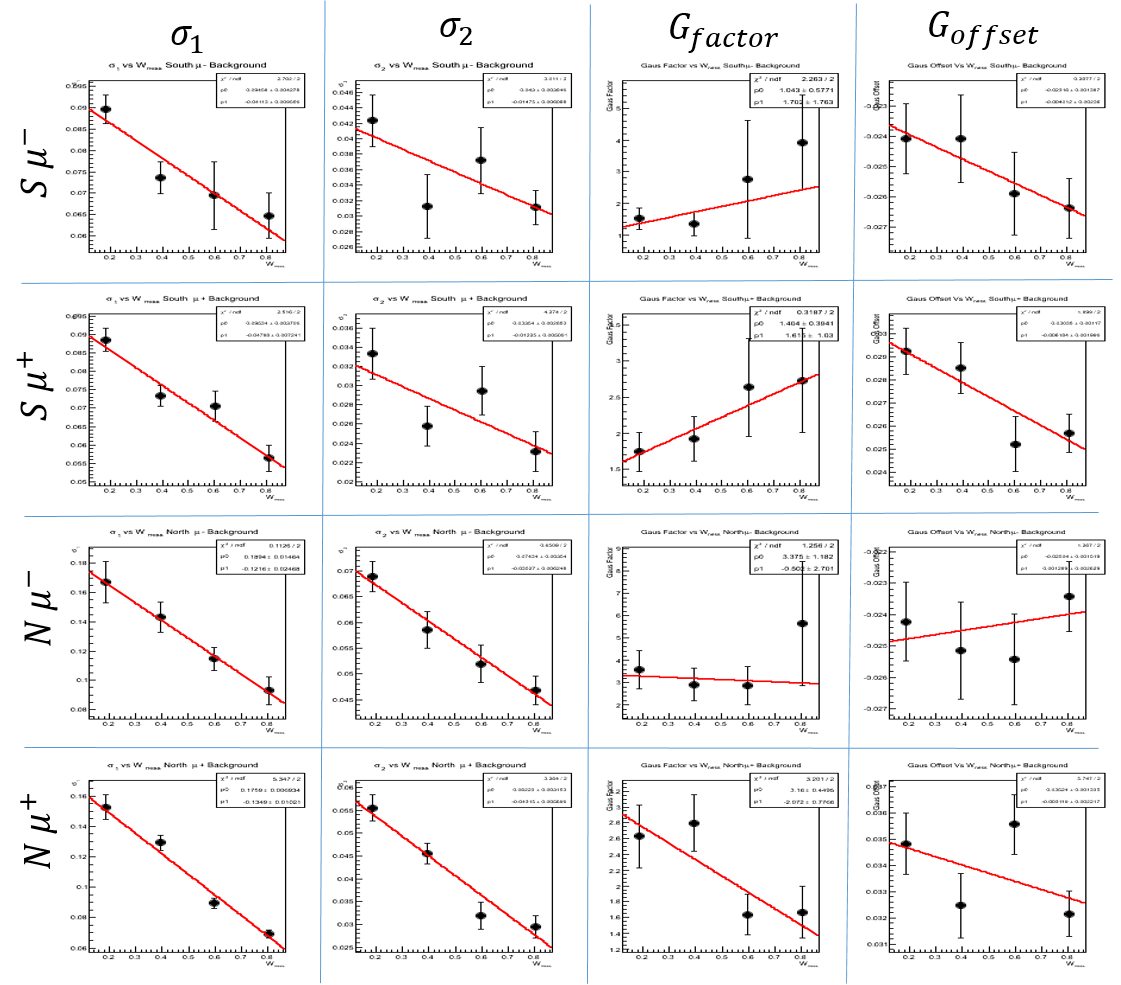
\includegraphics[width=\linewidth]{./figures/dw23_parameters_linearized.png}
  \caption{
    The four parameters from the co-axial Gaussian parameterization of $dw_{23}$
    as a function of $W_{ness}$. Though some parameters ($G_{factor}$, $N\mu-$)
    may appear to be non-linear, note that the uncertainty on some bins is quite
    large. Rows are arm/charge, labeled on the left, while columns are co-axial
    Gaussian parameters, summarized in Equation~\ref{eq:dw23_parameterization}
  }
  \label{fig:coax_params_vs_wness}
\end{figure}

The results of this fitting procedure are summarized in
Figure~\ref{fig:dw23_fits}.

\begin{figure}
  \centering
	\begin{subfigure}[t]{0.5\textwidth}
		\centering
    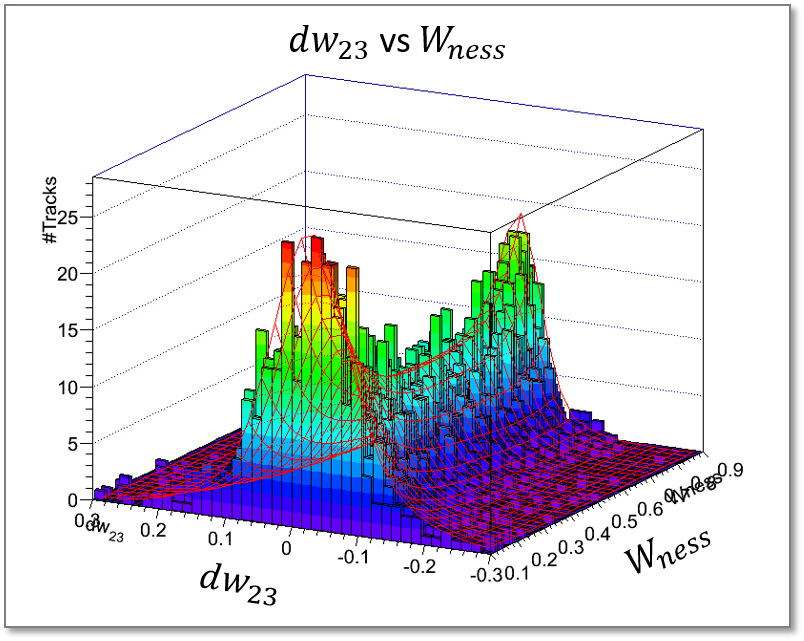
\includegraphics[width=0.95\linewidth]{./figures/dw23_vs_eta_3D.png}
    \caption{The final fit to $dw_{23}$ vs $W_{ness}$}
		\label{fig:3Ddw23_wness}
	\end{subfigure}%
  \begin{subfigure}[t]{0.5\textwidth}
		\centering
		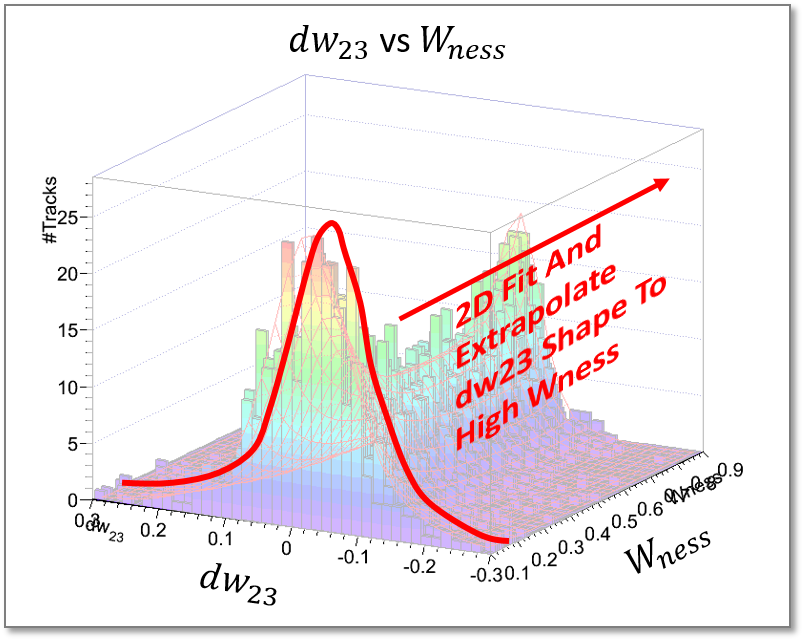
\includegraphics[width=0.95\linewidth]{./figures/dw23_vs_eta_3D_overlay.png}
    \caption{Cartoon of the extrapolation}
		\label{fig:3Ddw23_wness_overlay}
	\end{subfigure}
  \caption{
    The red wire-frame is the resultant fit of to the $dw_{23}$ vs $W_{ness}$
    distribution. We extrapolate the shape of $dw_{23}$ to the signal region to
    obtain the hadronic background PDF for $dw_{23}$.
  }
  \label{fig:dw23_fits}
\end{figure}

\begin{figure}
  \centering
  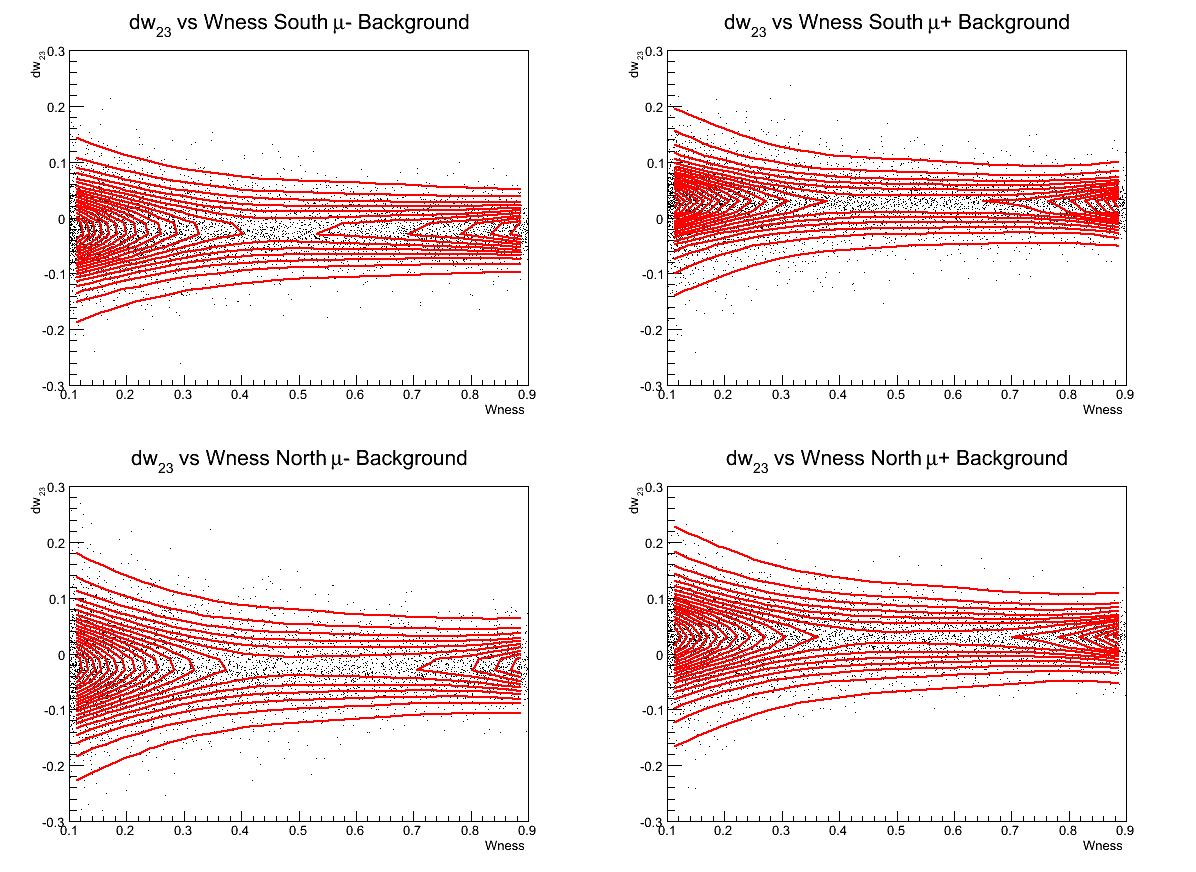
\includegraphics[width=\linewidth]{./figures/c_WnessVsdw23.png}
  \caption{
    An overhead view of the various results of the $dw_{23}$ vs $W_{ness}$ fit
    for each arm and charge combination.
  }
\end{figure}

Finally, the extrapolation of $dw_{23}$ was reproduced independently by four
separate analyzers, and cross-checked. The distributions are in close
agreement: Figure~\ref{fig:four_dw23}.

\begin{figure}
  \centering
  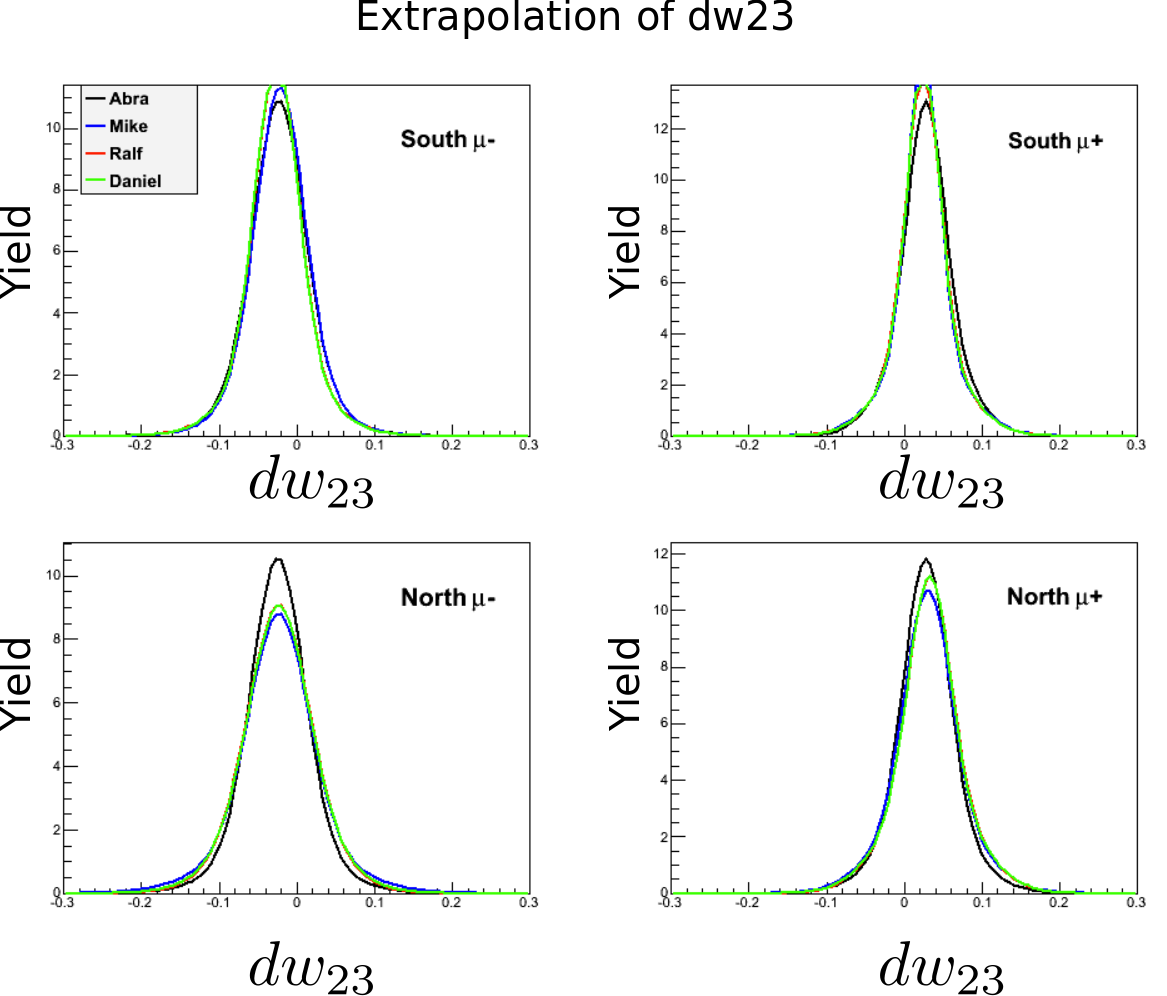
\includegraphics[width=0.7\linewidth]{./figures/dw23_fourway.png}
  \caption{
    Abraham, \textcolor{blue}{Mike}, \textcolor{red}{Ralf} and
    \textcolor{green}{Daniel} all independently parameterized and extrapolated
    $dw_{23}$ obtaining consistent results~\cite{Seidl2014a}.
  }
  \label{fig:four_dw23}
\end{figure}

The PDF for $\eta$ was obtained by creating a histogram of the variable for
events tagged with $W_{ness} < 0.9$. 

\clearpage
\subsection{Muon Background and W-Signal PDFs}

We have used the $W_{ness}$ cut to create a data set dominated by the
hadronic processes to form the hadronic background PDFs, we use simulations to
define the distributions for signal events and muon background events. This
portion of the analysis is constrained by our ability to reproduce accurate
representations of data sets which contain only signal events and muon
background events. We are confident in our ability to do this, due to the
physics mediating the production of these particles being well understood, in
addition to our high precision PISA models of the PHENIX detector geometry.

The muon background probability density functions and the W-Signal probability
density functions must be carefully summed from simulations so as to match the
likely composition of the data set. This is done by using the well known
cross-section of each of the processes which are simulated and normalizing with
the integrated luminosity delivered to PHENIX during the 2013 run of RHIC. This
luminosity was found to be $277 pb^{-1}$.

One caveat is that the minimum bias trigger of PHENIX is easily fooled by
effects such as pile-up and multiple collisions. Concretely, this occurs when
there is more than one collision in a single bunch crossing. This is typically
not a problem when PHENIX operates at lower energies and beam luminosities, but
for this data set, it was a real factor, that must be corrected for, else all
the ingredients in the muon background cocktail will be present in the wrong
amounts and we'll get the wrong answer from using them. Pile up refers to the
process where some events aren't read out quickly enough, and so one recorded
event will contain information for two actual beam crossings. Unaccounted for,
pile-up and multiple collisions both have the affect of lowering the measured
luminosity. 

The $277 pb^{-1}$ luminosity figure has been corrected for pile-up and multiple
collisions. This is a separate analysis, done by my colleagues working on this
analysis, so it will not be described in detail in this thesis, however it is
described in detail in our analysis note:~\cite{Seidl2014a}.

Finally, the PDFs used in the EULMF are shown in
Figures~\ref{fig:c_dw23_Eta_PDF_Arm0_Charge0}-\ref{fig:c_dw23_Eta_PDF_Arm1_Charge1}.

\begin{figure}
  \centering
  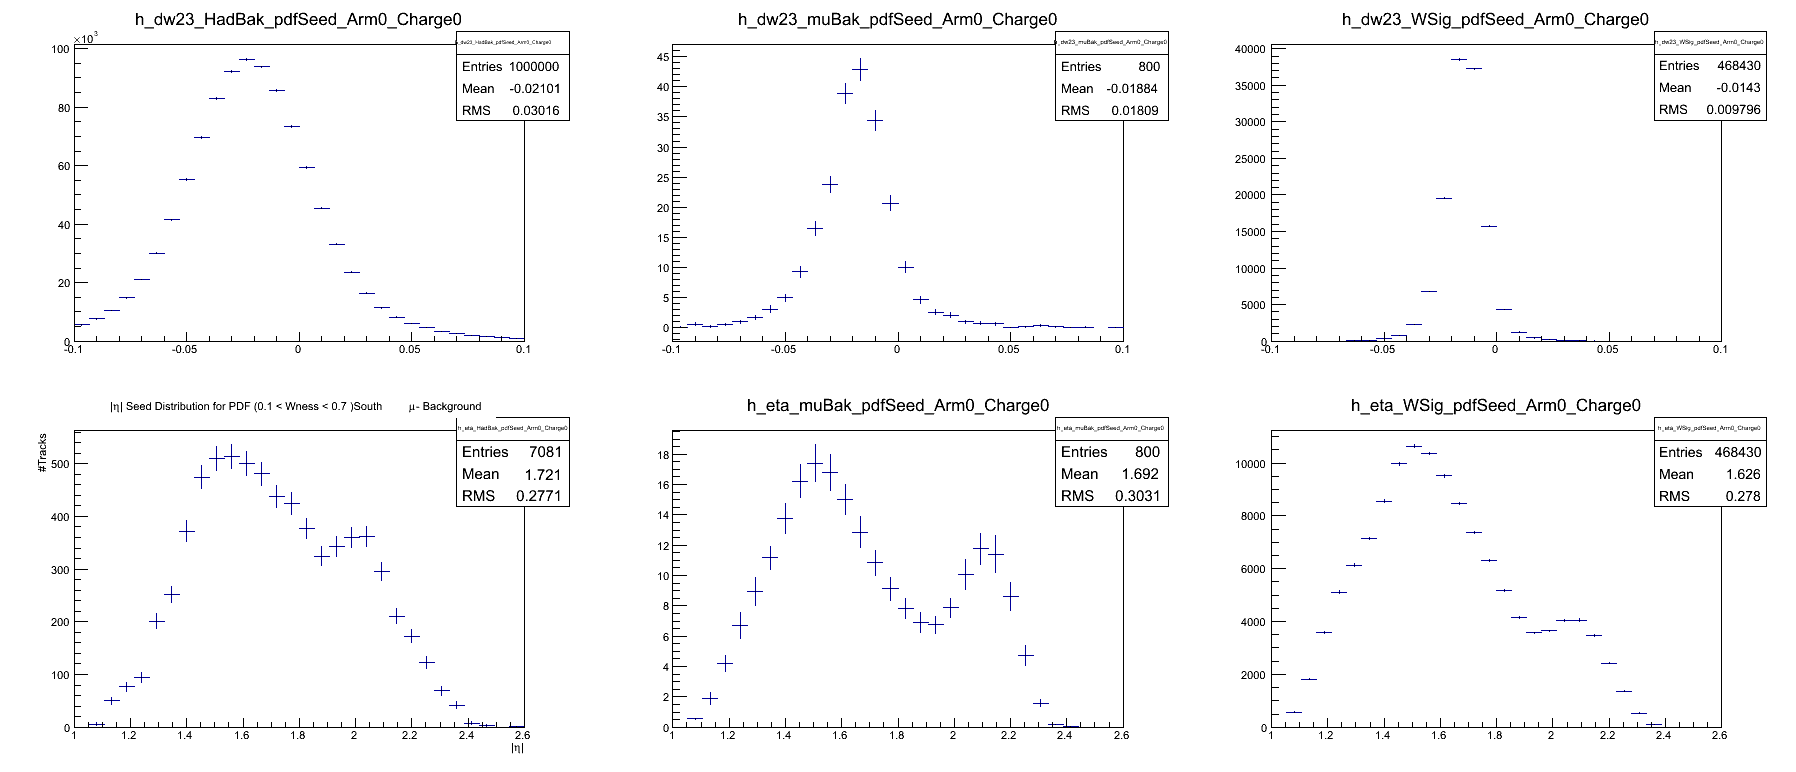
\includegraphics[width=\linewidth]{././figures/c_dw23_Eta_PDF_Arm0_Charge0.png}
  \caption{
    Left Column: The hadronic background PDFs, Middle Column: The Summed Muon
    Background PDFs, Right Column: The W-Signal PDF. For South Arm, $mu+$
  }
  \label{fig:c_dw23_Eta_PDF_Arm0_Charge0}
\end{figure}

\begin{figure}
  \centering
  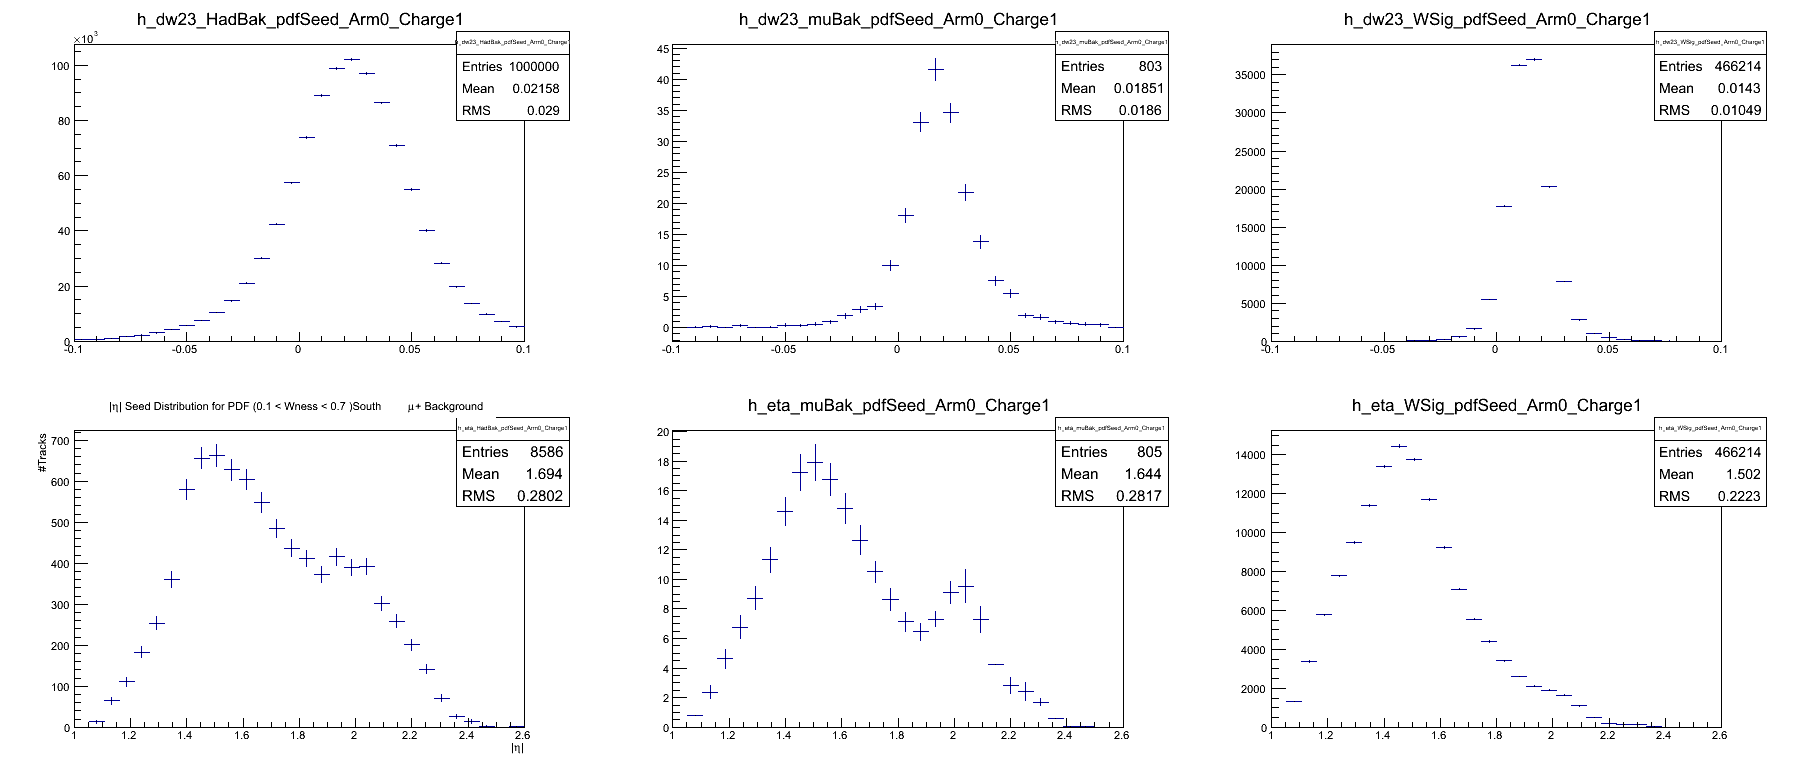
\includegraphics[width=\linewidth]{././figures/c_dw23_Eta_PDF_Arm0_Charge1.png}
  \caption{
    Left Column: The hadronic background PDFs, Middle Column: The Summed Muon
    Background PDFs, Right Column: The W-Signal PDF. For South Arm, $mu-$
  }
  \label{fig:c_dw23_Eta_PDF_Arm0_Charge1}
\end{figure}

\begin{figure}
  \centering
  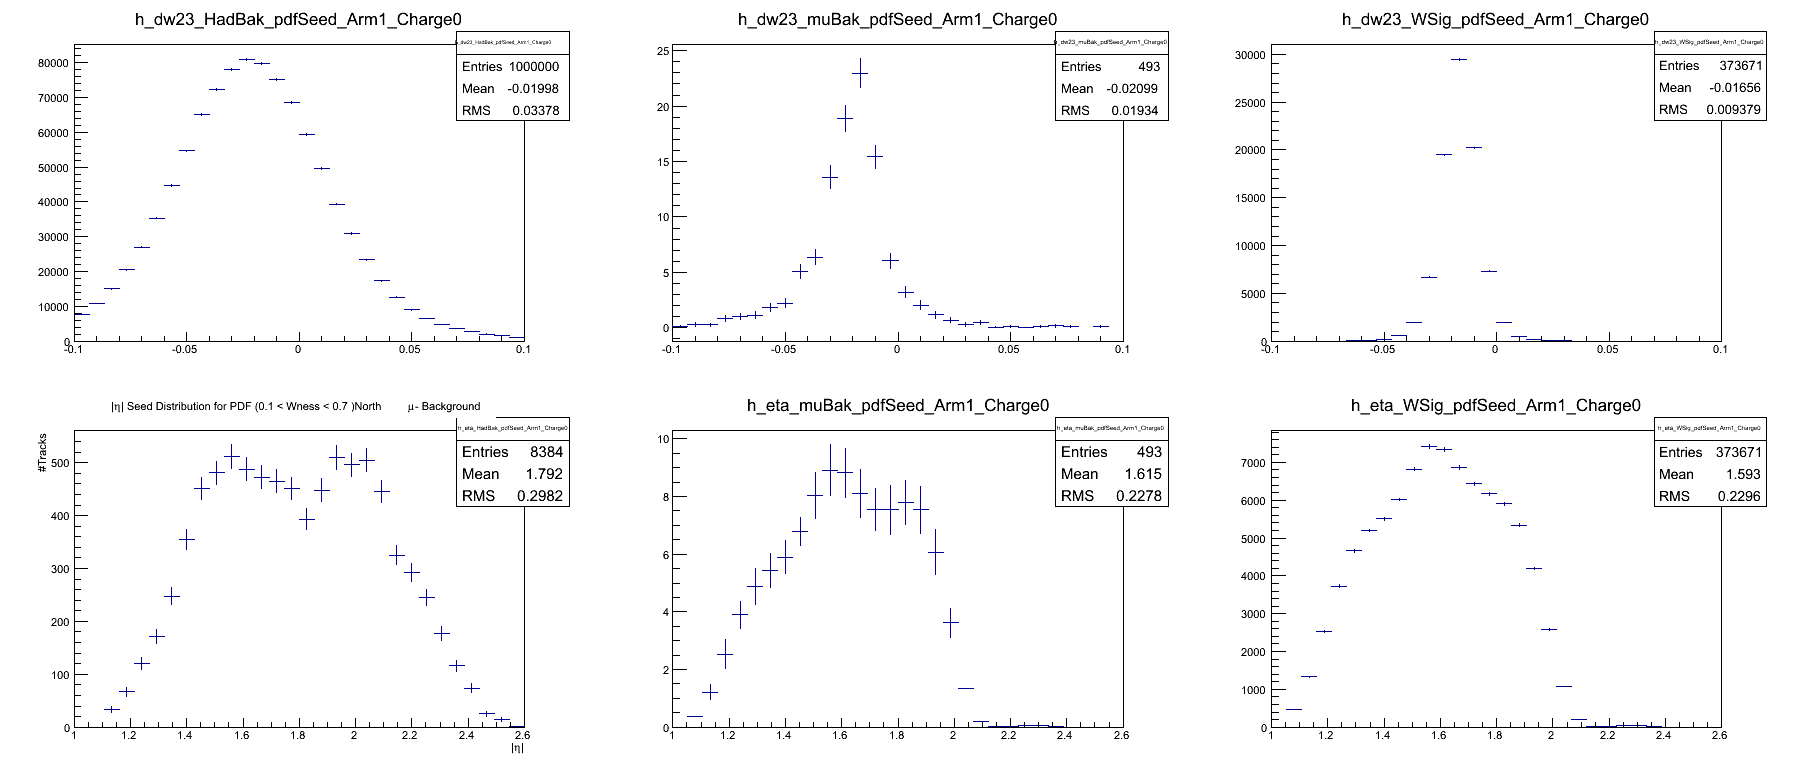
\includegraphics[width=\linewidth]{././figures/c_dw23_Eta_PDF_Arm1_Charge0.png}
  \caption{
    Left Column: The hadronic background PDFs, Middle Column: The Summed Muon
    Background PDFs, Right Column: The W-Signal PDF. For North Arm, $mu-$
  }
  \label{fig:c_dw23_Eta_PDF_Arm1_Charge0}
\end{figure}

\begin{figure}
  \centering
  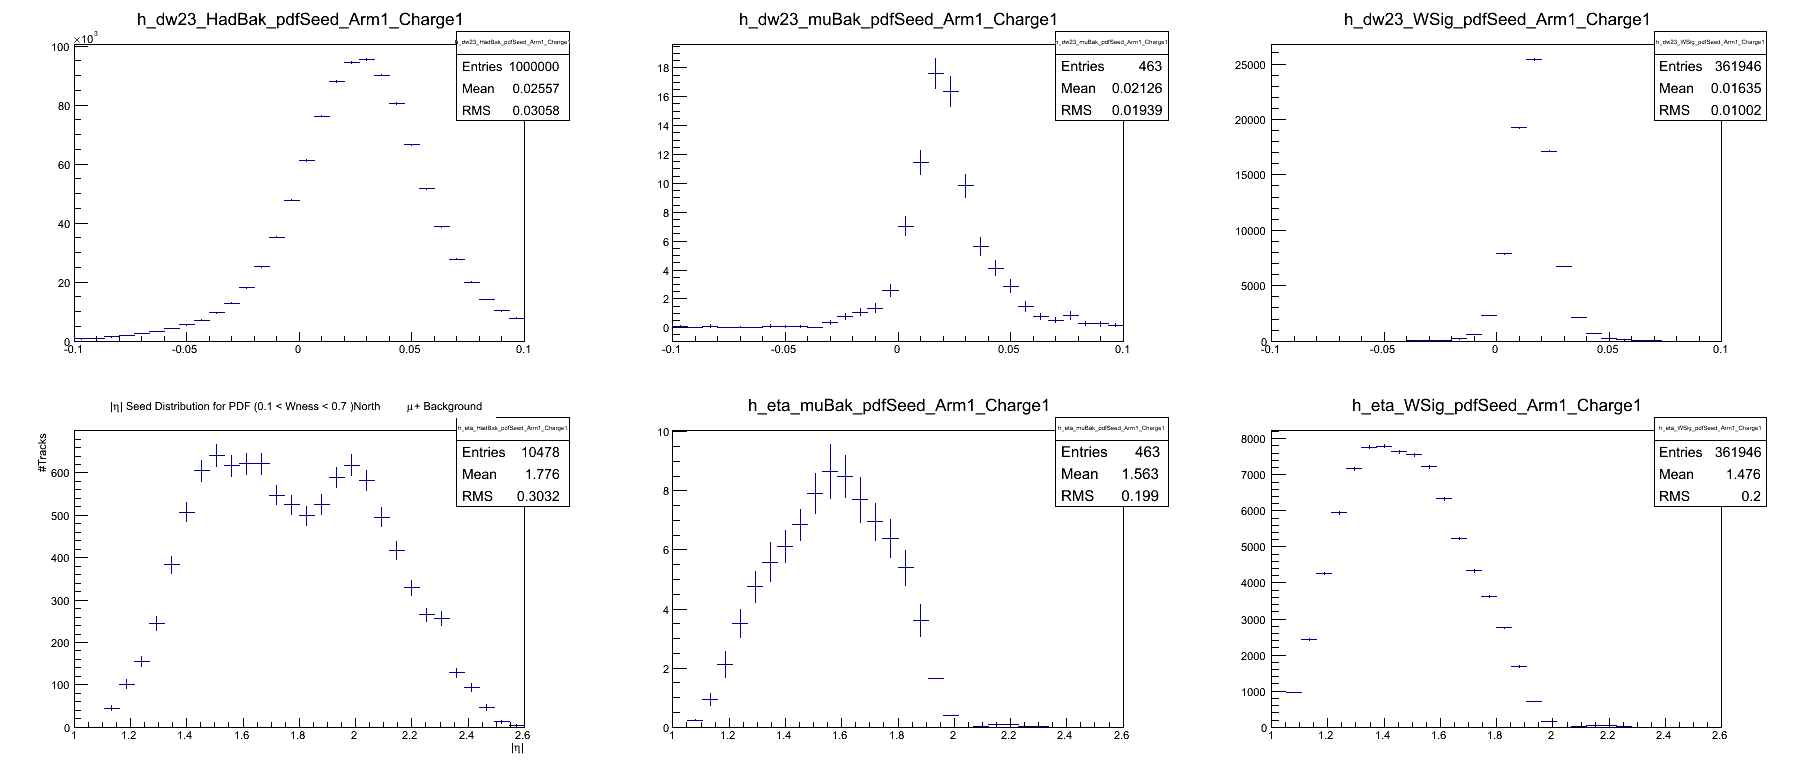
\includegraphics[width=\linewidth]{././figures/c_dw23_Eta_PDF_Arm1_Charge1.png}
  \caption{
    Left Column: The hadronic background PDFs, Middle Column: The Summed Muon
    Background PDFs, Right Column: The W-Signal PDF. For South Arm, $mu+$
  }
  \label{fig:c_dw23_Eta_PDF_Arm1_Charge1}
\end{figure}

With all PDFs prepared, we can perform the extended unbinned maximum likelihood
fit, and extract the yields for the number of signal muons, and the number of
fake hadronic background muons (recalling that the number of muon background
muons are fixed).

\begin{figure}
  \centering
  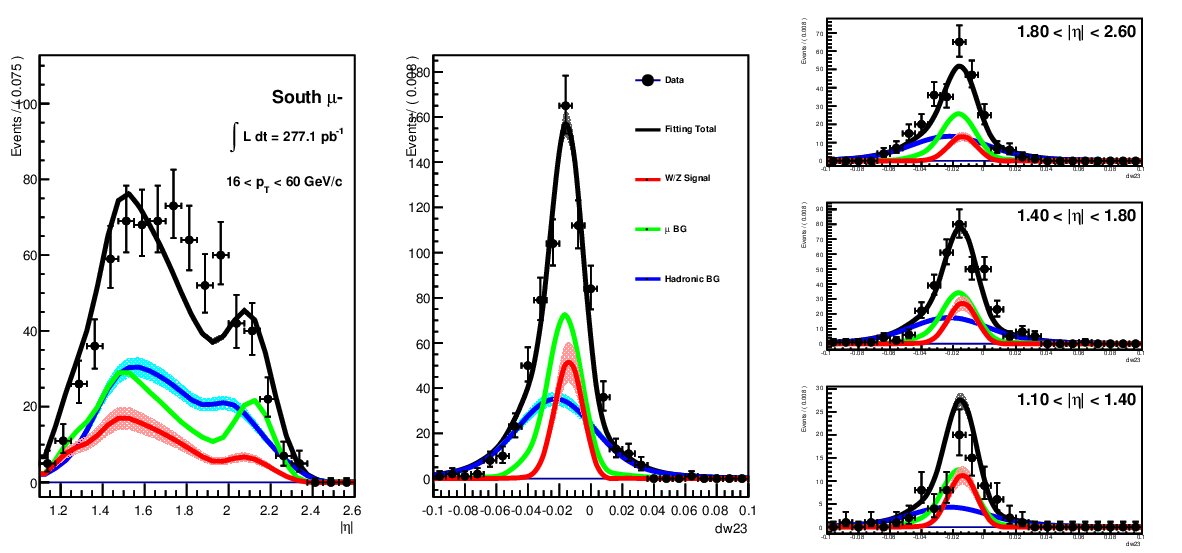
\includegraphics[width=\linewidth]{./figures/prelim_full_maxlikefit_a0q0.jpg}
  \caption{
    Here, we see the preliminary results of the EULMF for the 2013 Run. On the
    left, $\eta$ is shown. In the middle, $dw_{23}$. On the right, $dw_{23}$ is
    subdivided into the three standard $\eta$ bins. In all cases, we see the
    unbinned data in black (with error bars), and the sum of the three fits in
    black. In Blue, we can see the fake-muon hadronic background. In Green, the
    muon background. In blue, we see the W-Signal result. The area under the
    curves represents the yield, relative to the total. Shown: South Arm,
    $\mu-$~\cite{Seidl2014a}
  }
  \label{fig:maxlikefit_a0q0}
\end{figure}

\begin{figure}
  \centering
  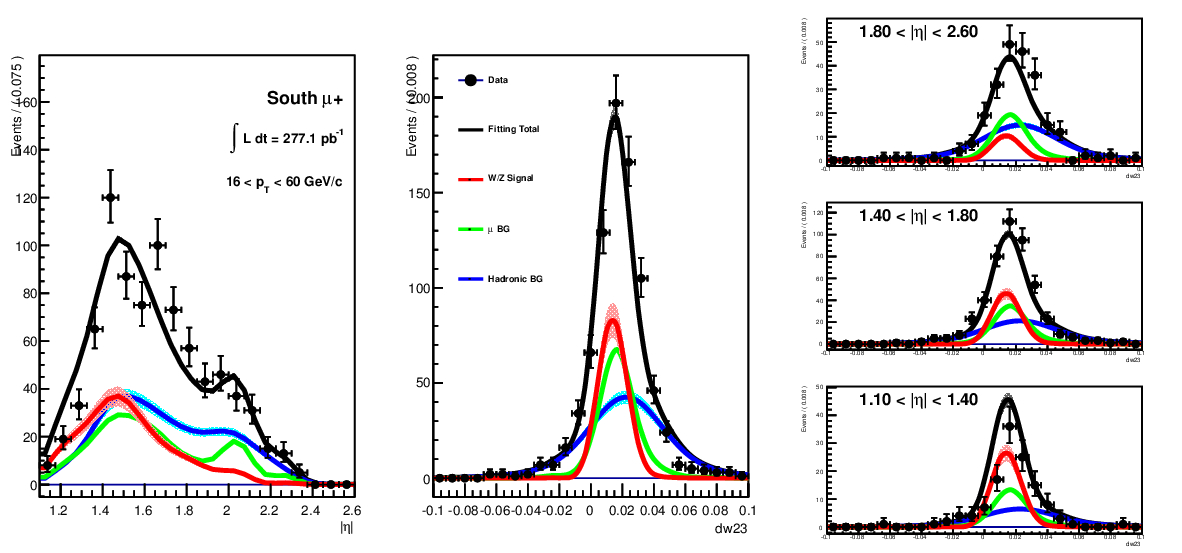
\includegraphics[width=\linewidth]{./figures/prelim_full_maxlikefit_a0q1.jpg}
  \caption{
    Here, we see the preliminary results of the EULMF for the 2013 Run. On the
    left, $\eta$ is shown. In the middle, $dw_{23}$. On the right, $dw_{23}$ is
    subdivided into the three standard $\eta$ bins. In all cases, we see the
    unbinned data in black (with error bars), and the sum of the three fits in
    black. In Blue, we can see the fake-muon hadronic background. In Green, the
    muon background. In blue, we see the W-Signal result. The area under the
    curves represents the yield, relative to the total.  Shown: South Arm,
    $\mu+$~\cite{Seidl2014a}
  }
  \label{fig:maxlikefit_a0q1}
\end{figure}

\begin{figure}
  \centering
  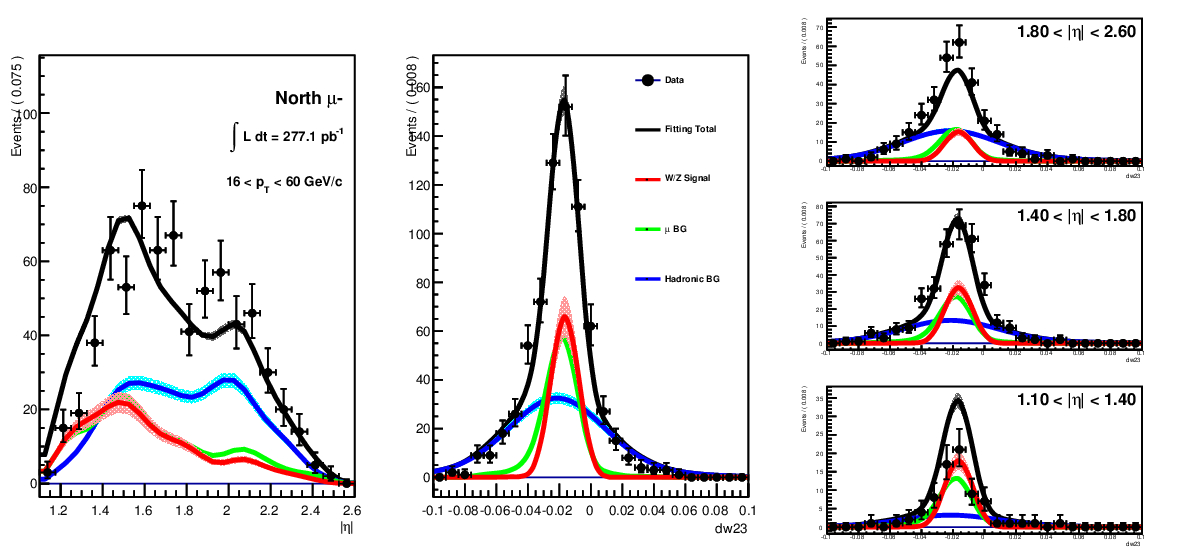
\includegraphics[width=\linewidth]{./figures/prelim_full_maxlikefit_a1q0.jpg}
  \caption{
    Here, we see the preliminary results of the EULMF for the 2013 Run. On the
    left, $\eta$ is shown. In the middle, $dw_{23}$. On the right, $dw_{23}$ is
    subdivided into the three standard $\eta$ bins. In all cases, we see the
    unbinned data in black (with error bars), and the sum of the three fits in
    black. In Blue, we can see the fake-muon hadronic background. In Green, the
    muon background. In blue, we see the W-Signal result. The area under the
    curves represents the yield, relative to the total.  Shown: North Arm,
    $\mu-$~\cite{Seidl2014a}
  }
  \label{fig:maxlikefit_a1q0}
\end{figure}

\begin{figure}
  \centering
  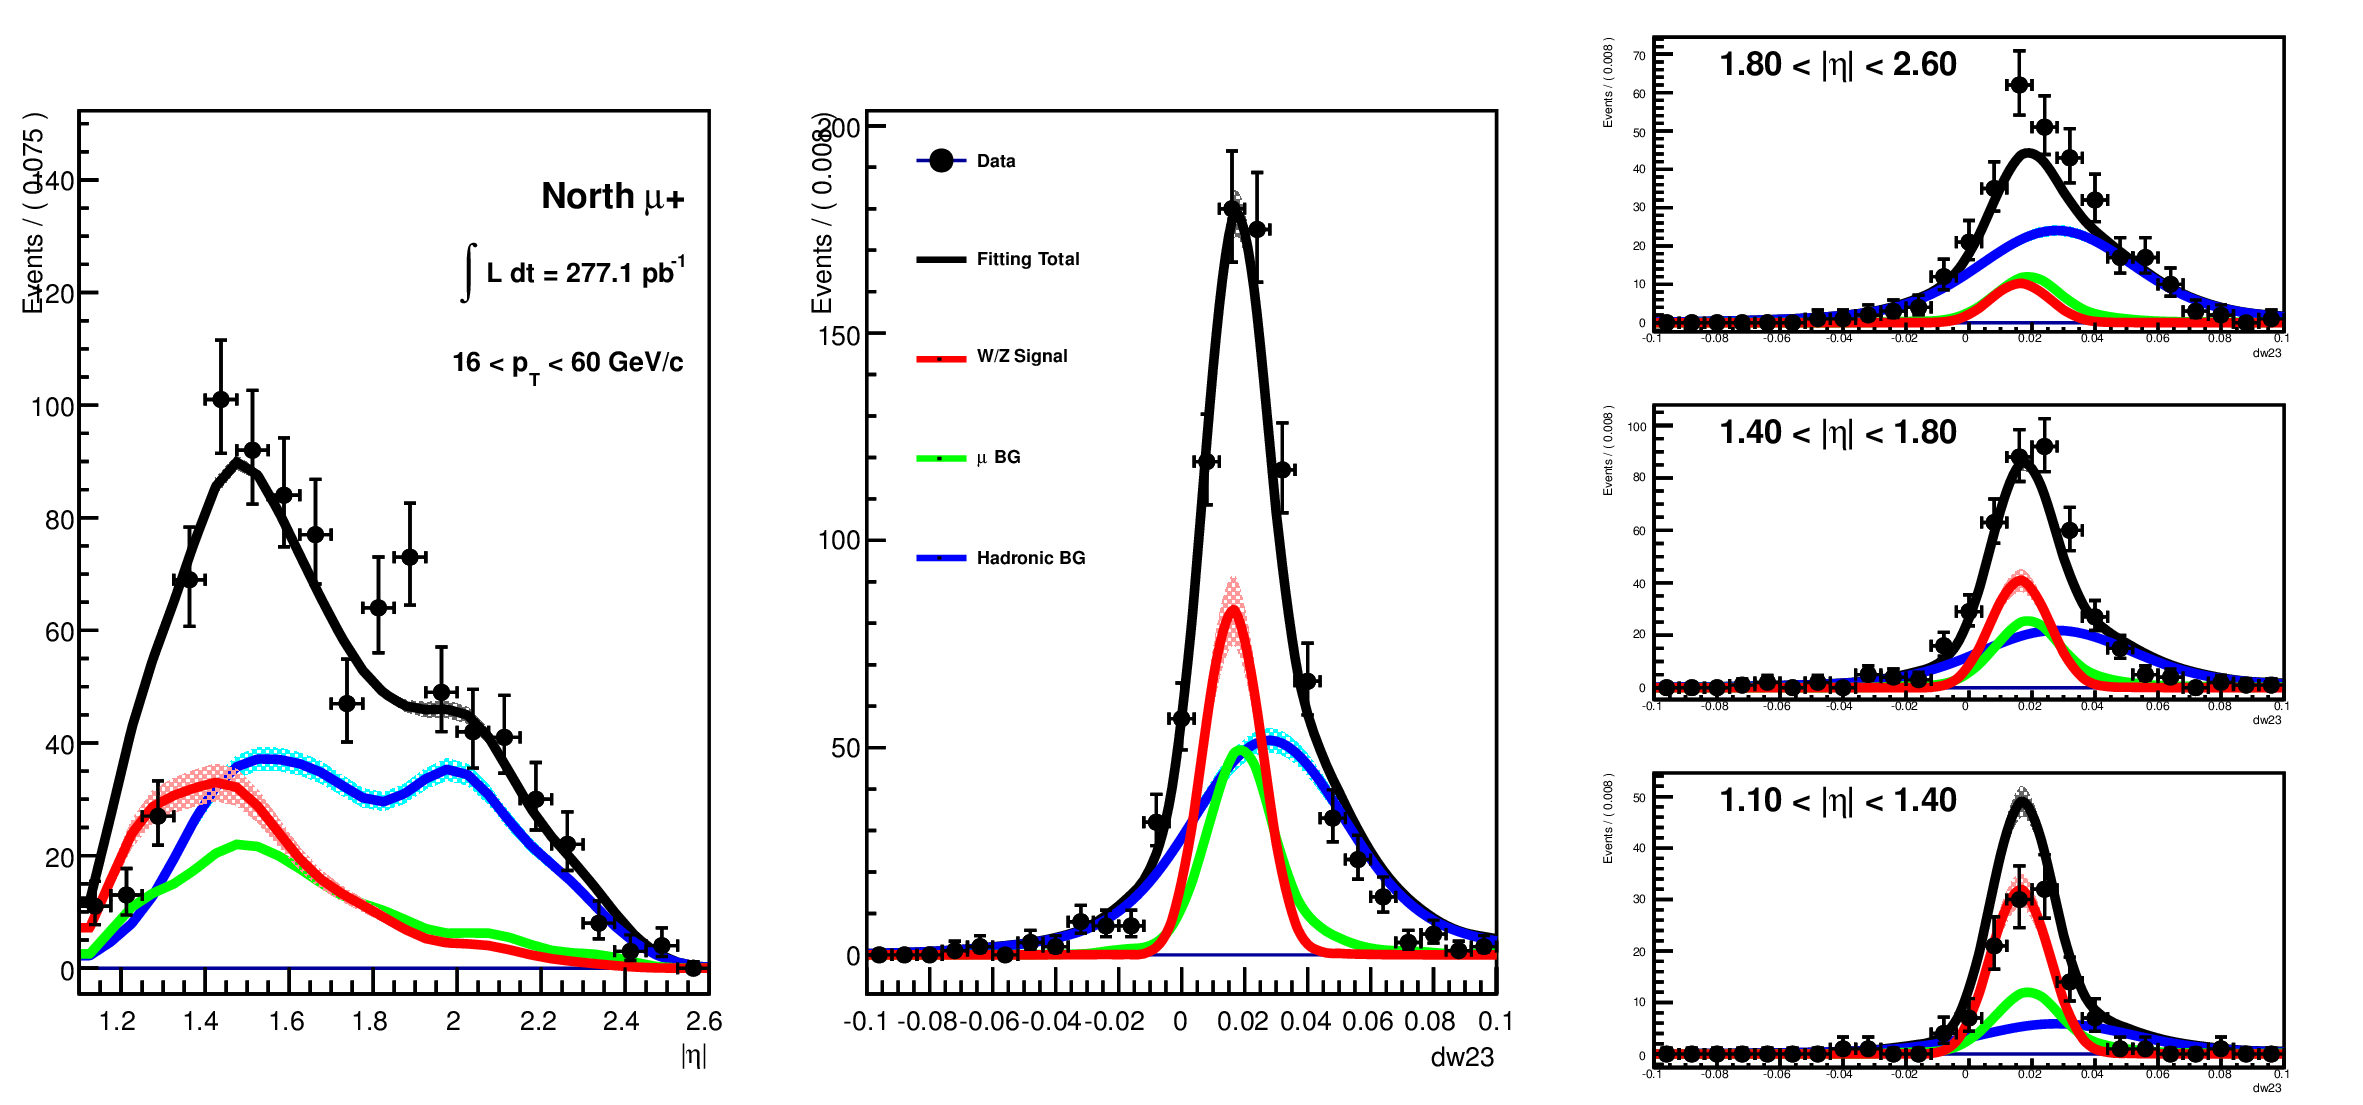
\includegraphics[width=\linewidth]{./figures/prelim_full_maxlikefit_a1q1.jpg}
  \caption{
    Here, we see the preliminary results of the EULMF for the 2013 Run. On the
    left, $\eta$ is shown. In the middle, $dw_{23}$. On the right, $dw_{23}$ is
    subdivided into the three standard $\eta$ bins. In all cases, we see the
    unbinned data in black (with error bars), and the sum of the three fits in
    black. In Blue, we can see the fake-muon hadronic background. In Green, the
    muon background. In blue, we see the W-Signal result. The area under the
    curves represents the yield, relative to the total. Shown: North Arm,
    $\mu+$~\cite{Seidl2014a}.
  }
  \label{fig:maxlikefit_a1q1}
\end{figure}

The signal to background ratio extraction is summarized by each analyzer in
Table~\ref{tab:sbr_per_analyzer}, for the South Arm $\mu-$ (the canonical
cross check).

\begin{table}[h]
  \centering
  \resizebox{\textwidth}{!}{\begin{tabular}{c|rrrr}
    \toprule
    \multicolumn{5}{c}{\textbf{South $\mu ^{-}$}}  \\  
    \textbf{Variable} & \textbf{Ralf} & \textbf{Daniel} & \textbf{Mike} &
    \textbf{Abraham} \\  
    \midrule
    \textbf{Total events} & $    2032$&$    2034$&$     2022$&$     2039$\\ 
    \textbf{Signal events} & $     340^{+42.14} _{-41.42}$&$      303^{+42.31} _{-41.59}$&$      332^{+42.28} _{-41.58}$&$      294^{+41.38} _{-41.38}$\\ 
    \textbf{Hadron events} & $    1424^{+53.57} _{-52.60}$&$     1469^{+54.55} _{-53.59}$&$     1433^{+53.97} _{-52.99}$&$     1485^{+53.85} _{-53.85}$\\ 
    \textbf{Muon events} & $     269$&$     262$&$      257$&$      259$\\  
    \textbf{Signal/BG} & $    0.20^{+0.03} _{-0.03}$&$     0.18^{+0.00} _{-0.00}$&$     0.20^{+0.03} _{-0.03}$&$     0.17^{+0.02} _{-0.00}$\\ 
    \bottomrule
\end{tabular}}
  \caption{ South arm $W\rightarrow \mu^{-}$ fit results per analyzer
  ~\cite{Seidl2014a}}
  \label{tab:sbr_per_analyzer}
\end{table}
\clearpage

\begin{sidewaystable}
  \centering
  \resizebox{\textwidth}{!}{\begin{tabular}{llccccc}
      \toprule
      \textbf{Arm} & 
      \textbf{Charge} & 
      \textbf{Total Events} & 
      \textbf{Signal Events} & 
      \textbf{Fake Muons} & 
      \textbf{Muon Background} & 
      \textbf{SBR} \\
      \midrule
      S & $\mu-$ & 2023 & $354^{+41.9714}_{-41.2598}$ & $1448^{53.6777}_{-52.7162}$ & $221^{0.212103}_{0.0263482}$ & 0.0258992 \\
      S & $\mu+$ & 2468 & $498^{+44.0941}_{-43.2297}$ & $1767^{57.046 }_{-56.3006}$ & $203^{0.252792}_{0.0238242}$ & 0.0233755 \\
      N & $\mu-$ & 2029 & $370^{+34.4599}_{-33.7046}$ & $1555^{48.5042}_{-47.6586}$ & $104^{0.223026}_{0.0219055}$ & 0.0214353 \\
      N & $\mu+$ & 2633 & $505^{+37.9628}_{-37.2192}$ & $2043^{54.5676}_{-53.7571}$ & $85 ^{0.237312}_{0.0189323}$ & 0.0185715 \\
      \bottomrule
  \end{tabular}}
  \caption{ 
    A summary table from the results of the EULMF to the unbinned data set,
    summed to one $\eta$ bin per arm and charge.
  }
\end{sidewaystable}

\section{Systematic Tests}

One of the rare advantages of this analysis was that I had the opportunity to
undertake it in parallel with others, working as a team to accomplish our goals.
That means that we were able perform many systematic tests. These tests are
summarized in the Appendix~\ref{appendix_1}, and serve to lend confidence to our
extraction of the signal to background ratio.
